\chapter{Strong-production multi-b SUSY search}
\label{chap:strong_prod}


\section{Signal model}

The simplified models used to optimize this analysis are the two gluino-pair-production models shown in Fig. \ref{fig:strong_diagram}. 
Figure \ref{fig:diagram_Gtt} shows a schematic diagram of the Gtt model: 
each of the pair-produced gluinos decays with 100\% \gls{br} to two top quarks and the lightest neutralino (\ninoone).
In the Gbb model, shown in Figure \ref{fig:diagram_Gbb}, the decay happens through an off-shell sbottom and each gluino transforms into 
two bottom quarks and the \ninoone. Both models assume R-parity conservation, so the \ninoone, which in this case is the \gls{lsp} is stable 
and escapes undetected, giving rise to \met in the event. In both cases, the three body decay is realized through an off-shell squark, 
and it involves two interaction vertexes. The first one is a strong-interaction vertex, in the case of the Gtt model:

\begin{equation*}
\gluino \to t \stop^{(*)} \; .
\end{equation*}

\noindent The second is an electroweak vertex, originating from the decay of the \stop (or \sbottom in the case of the Gbb model):

\begin{equation*}
\stop \to t \ninoone
\end{equation*}

\begin{figure*}[h]
\centering 
\subfigure[]{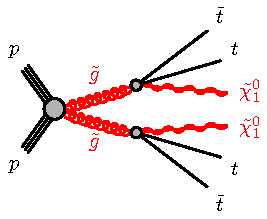
\includegraphics[width=0.35\textwidth]{figures/strong_prod/diagrams/gogo-ttttN1N1.pdf}\label{fig:diagram_Gtt}}
\subfigure[]{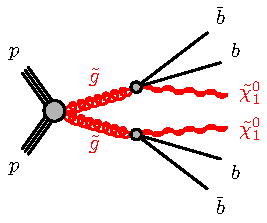
\includegraphics[width=0.35\textwidth]{figures/strong_prod/diagrams/gogo-bbbbN1N1.pdf}\label{fig:diagram_Gbb}}
\caption{The simplified models used for the optimization of the analysis. \subref{fig:diagram_Gtt} Gtt model. \subref{fig:diagram_Gbb} Gbb model.
}\label{fig:strong_diagram}
\end{figure*}

In the Gtt and Gbb models, since the \stop and \sbottom are assumed to have very high mass, the only parameters are the mass and production cross section of the gluino, and the mass of the \gls{lsp}. While the Gtt and Gbb models are used both to optimize and interpret the analysis, a further interpretation is provided also in terms of a slightly more complicated model. If we allow also the lightest chargino (\chinoonepm) to have a reachable mass, another decay chain opens, where the virtual stop or sbottom decays to a \chinoonepm:

\begin{equation*}
\begin{split}
\stop &\to \bar{b} \chinoonem \; , \\
\sbottom &\to t \chinoonem \; .
\end{split}
\end{equation*}  

The charge-conjugate processes are also possible, and in both cases the overall decay chain of the gluino leads to $\gluino \to t b \chinoonem$, which we refer to as Gtb model.
The model used to re-interpret this analysis assumes the decay $\chinoonepm \to \ninoone W^{\pm}$, where the W boson can be off-shell if the mass difference between the \chinoonepm and the \ninoone is not large enough to produce an on-shell W boson. 
This mass difference becomes a further parameter of the model. The model considered in this analysis assumes that the \chinoonepm and the \ninoone 
are almost degenerate (in the \gls{mc} simulation, they are generated with a mass difference of 2 GeV); in this case the W boson is virtual and results into soft fermions, that most of the time are not reconstructed. This small difference is often verified in models where the \chinoonepm and the \ninoone are part of an approximate $SU(2)$ multiplet, and setting it to a fixed value allows to reduce the number of parameters of the model. 
This analysis provides an interpretation of the result in terms of \gls{br} of the gluino into the Gtt, Gbb and Gtb models. 
A schematic diagram of the possible decay chains in this mixed-\gls{br} interpretation, in addition to the ones shown in Fig. \ref{fig:strong_diagram}, is shown in Fig. \ref{fig:strong_diagram_br}.

\begin{figure*}[h]
\centering 
\subfigure[]{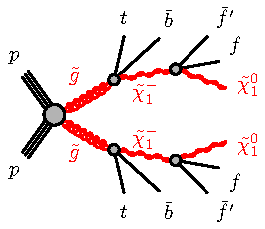
\includegraphics[width=0.35\textwidth]{figures/strong_prod/diagrams/gogo-tbfftbffN1N1.pdf}\label{fig:diagram_strong_tbtb}}
\subfigure[]{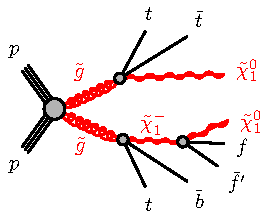
\includegraphics[width=0.35\textwidth]{figures/strong_prod/diagrams/gogo-tttbffN1N1.pdf}\label{fig:diagram_strong_tttb}}\\
\subfigure[]{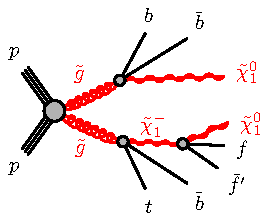
\includegraphics[width=0.35\textwidth]{figures/strong_prod/diagrams/gogo-bbtbffN1N1.pdf}\label{fig:diagram_strong_bbtb}}
\subfigure[]{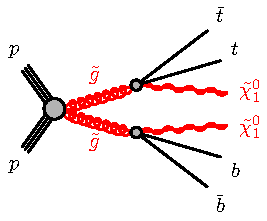
\includegraphics[width=0.35\textwidth]{figures/strong_prod/diagrams/gogo-ttbbN1N1.pdf}\label{fig:diagram_strong_ttbb}}
\caption{Simplified models used in the re-interpretation of the analysis. \subref{fig:diagram_strong_tbtb} Both gluinos have the following decay chain: $\gluino \to t \bar{b} \chinoonem$ with $\chinoonem \to f\bar{f}' \ninoone$. \subref{fig:diagram_strong_tttb} One gluino decays as in \subref{fig:diagram_strong_tbtb} and the other as $\gluino \to t\bar{t}\ninoone$. \subref{fig:diagram_strong_bbtb} One gluino decays as in \subref{fig:diagram_strong_tbtb} and the other as $\gluino \to b\bar{b}\ninoone$. \subref{fig:diagram_strong_ttbb} One gluino decays as $\gluino \to t\bar{t}\ninoone$ and the other as $\gluino \to b\bar{b}\ninoone$.  %The charge conjugate processes are implied.
%The fermions originating from the $\chinoonepm$ decay are typically soft because the mass difference  between the $\chinoonepm$ and the $\ninoone$ is fixed to 2 GeV. 
}\label{fig:strong_diagram_br}
\end{figure*}


These gluino decay chains that lead to final states rich in heavy-flavour quarks are dominant in \gls{susy} models where the squarks 
from the first two generations are significantly heavier than stop and sbottom, or also in cases when the \ninoone is dominated by the higgsino component. 

\section{Previous limits}

\section{Kinematic variables specific to this analysis}

\subsubsection*{Total jet mass}

\begin{equation}
\mjsum = \sum_{i \leq 4} m_{J,i}
\end{equation}

\subsubsection*{ISR jet}

\begin{equation}
|{\Delta}{\phi}(j1, \met)|
\end{equation}



\section{Pre-fit data-MC}


\section{Discovery signal regions}

\begin{table}[t]
    \centering
 \renewcommand{\arraystretch}{1.5}
   \caption{Definitions of the Gtt SRs, CRs and VRs of the cut-and-count analysis.  All kinematic variables are
   expressed in \gev\ except $\dphimin$, which is in radians. The jet \pt\ requirement is also applied to 
   $b$-tagged jets.}
   \label{tab:GttEvsel}
         \begin{tabular}{c c c c c c c c}
        \toprule
\multicolumn{8}{c}{\textbf{ Gtt 1-lepton}}\\
\multicolumn{8}{c}{Criteria common to all regions: $\ge 1$ signal lepton, ${\pt}^\mathrm{jet} >  30~\gev$, $\nbjet \geq 3$} \\\midrule
Targeted kinematics & Type & $\njet$ & $\mt$ & $\mtb$& $\met$ & $\meffi$ & $\mjsum$ \\ \midrule
\multirow{4}{*}{\begin{minipage}{3cm}\centering Region B\\
              (Boosted, Large \msplit) \end{minipage}} 
 & SR & $\ge 5$ & $> 150$ & $> 120 $  & $> 500 $ & $> 2200 $ & $> 200$  \\
 & CR & $= 5$ & $< 150$ & $-$  & $> 300 $ & $> 1700 $ & $> 150$  \\
 & VR-$\mt$ & $\ge 5$ & $> 150$ & $-$  & $> 300 $ & $> 1600 $ & $< 200$  \\
& VR-$\mtb$ & $> 5$ & $< 150$ & $> 120 $  & $> 400 $ & $> 1400 $ & $> 200$  \\\midrule
\multirow{4}{*}{\begin{minipage}{3cm}\centering Region M\\
              (Moderate \msplit) \end{minipage}} 
 & SR & $\ge 6$ & $> 150$ & $> 160 $  & $> 450 $ & $> 1800 $ & $> 200$  \\
 & CR & $= 6$ & $< 150$ & $-$  & $> 400 $ & $> 1500 $ & $> 100$  \\
 & VR-$\mt$ & $\ge 6$ & $> 200$ & $-$  & $> 250 $ & $> 1200 $ & $< 100$  \\
& VR-$\mtb$ & $> 6$ & $< 150$ & $> 140 $  & $> 350 $ & $> 1200 $ & $> 150$  \\\midrule
\multirow{4}{*}{\begin{minipage}{3cm}\centering Region C\\
              (Compressed, small \msplit) \end{minipage}} 
 & SR & $\ge 7$ & $> 150$ & $> 160 $  & $> 350 $ & $> 1000 $ & $-$  \\
 & CR & $= 7$ & $< 150$ & $-$  & $> 350 $ & $> 1000 $ & $-$  \\
 & VR-$\mt$ & $\ge 7$ & $> 150$ & $< 160 $  & $> 300 $ & $> 1000 $ & $-$  \\
& VR-$\mtb$ & $> 7$ & $< 150$ & $> 160 $  & $> 300 $ & $> 1000 $ & $-$  \\
      \end{tabular}
         \begin{tabular}{c c c c c c c c c c c}
        \toprule
\multicolumn{11}{c}{\textbf{ Gtt 0-lepton}}\\
\multicolumn{11}{c}{Criteria common to all regions: ${\pt}^\mathrm{jet} > 30$~GeV} \\\midrule
Targeted kinematics & Type & $N_\mathrm{lepton}$ & $\nbjet$& $\njet$&  $\dphimin$ & $\mt$ & $\mtb$ & $\met$ & $\meffi$ & $\mjsum$ \\ \midrule
\multirow{3}{*}{\begin{minipage}{3cm}\centering Region B\\
              (Boosted, Large \msplit) \end{minipage}} 
& SR & $= 0$  & $\ge 3$ & $\ge 7$ & $>0.4$ & $-$ & $> 60 $ & $> 350 $ & $> 2600$ & $> 300$\\ 
& CR & $= 1$  & $\ge 3$ & $\ge 6$ & $-$ & $<150$ & $-$ & $> 275 $ & $> 1800$ & $> 300$\\ 
& VR & $= 0$  & $\ge 3$ & $\ge 6$ & $>0.4$ & $-$ & $-$ & $> 250 $ & $> 2000$ & $< 300$\\ \midrule
\multirow{3}{*}{\begin{minipage}{3cm}\centering Region M\\
              (Moderate \msplit) \end{minipage}} 
& SR & $= 0$  & $\ge 3$ & $\ge 7$ & $>0.4$ & $-$ & $> 120 $ & $> 500 $ & $> 1800$ & $> 200$\\ 
& CR & $= 1$  & $\ge 3$ & $\ge 6$ & $-$ & $<150$ & $-$ & $> 400 $ & $> 1700$ & $> 200$\\ 
& VR & $= 0$  & $\ge 3$ & $\ge 6$ & $>0.4$ & $-$ & $-$ & $> 450 $ & $> 1400$ & $< 200$\\ \midrule
\multirow{3}{*}{\begin{minipage}{3cm}\centering Region C\\
              (Compressed, moderate \msplit) \end{minipage}} 
& SR & $= 0$  & $\ge 4$ & $\ge 8$ & $>0.4$ & $-$ & $> 120 $ & $> 250 $ & $> 1000$ & $> 100$\\ 
& CR & $= 1$  & $\ge 4$ & $\ge 7$ & $-$ & $<150$ & $-$ & $> 250 $ & $> 1000$ & $> 100$\\ 
& VR & $= 0$  & $\ge 4$ & $\ge 7$ & $>0.4$ & $-$ & $-$ & $> 250 $ & $> 1000$ & $< 100$\\ 

        \bottomrule
      \end{tabular}
 \end{table}


\clearpage



\begin{landscape}
\begin{table}[t]
    \centering
 \renewcommand{\arraystretch}{1.3}
%   \caption{Definitions of the Gbb SRs, CRs and VRs of the cut-and-count analysis.  All kinematic variables are
%   expressed in \gev\ except $\dphimin$, which is in radians. The jet \pt\ requirement is applied to the 
%   four leading jets, a subset of which are $b$-tagged jets. The $\leadjet \neq b$  requirement specifies that 
%   the leading jet is not $b$-tagged.}
    \label{tab:Gbb0LEvsel}
         \begin{tabular}{c c c c c c c c c c}
        \toprule
\multicolumn{10}{c}{\textbf{ Gbb}}\\
\multicolumn{10}{c}{Criteria common to all regions: $\njet \geq 4$,
           ${\pt}^\mathrm{jet} > 30$~GeV } \\\midrule 
Targeted kinematics  & Type & $N_\mathrm{lepton}$ & $\nbjet$ &  $\dphimin$ & $\mt$ & $\mtb$ & $\met$ & $\meff$ & Others  \\\midrule
\multirow{3}{*}{\begin{minipage}{3cm}\centering Region B\\
              (Boosted, Large \msplit) \end{minipage}} 
& SR & $= 0$  & $\ge 3$ & $>0.4$ & $-$ & $- $ & $> 400 $ & $> 2800$ & $-$ \\ 
& CR & $= 1$  & $\ge 3$ & $-$ & $< 150$ & $- $ & $> 400 $ & $> 2500$ & $-$ \\ 
& VR & $= 0$  & $\ge 3$ & $>0.4$ & $-$ & $- $ & $> 350 $ & $1900$--$2800$ & $-$ \\\midrule
\multirow{3}{*}{\begin{minipage}{3cm}\centering Region M\\
              (Moderate \msplit) \end{minipage}} 
& SR & $= 0$  & $\ge 4$ & $>0.4$ & $-$ & $>90$ & $> 450 $ & $> 1600$ & $-$ \\ 
& CR & $= 1$  & $\ge 4$ & $-$ & $< 150$ & $- $ & $> 300 $ & $> 1600$ & $-$ \\ 
& VR & $= 0$  & $\ge 4$ & $>0.4$ & $-$ & $>100$ & $250$--$450$ & $1600$--$1900$ & $-$ \\\midrule
\multirow{3}{*}{\begin{minipage}{3cm}\centering Region C\\
              (Compressed, small \msplit) \end{minipage}} 
& SR & $= 0$  & $\ge 4$ & $>0.4$ & $-$ & $>155$ & $> 450 $ & $-$ & $-$ \\ 
& CR & $= 1$  & $\ge 4$ & $-$ & $< 150$ & $- $ & $> 375 $ & $-$ & $-$ \\ 
& VR & $= 0$  & $\ge 4$ & $>0.4$ & $-$ & $>125$ & $350$--$450$ & $-$ & $-$ \\\midrule
\multirow{3}{*}{\begin{minipage}{3cm}\centering Region VC\\
              (Very Compressed, very small \msplit) \end{minipage}} 
& SR & $= 0$  & $\ge 3$ & $>0.4$ & $-$ & $>100$ & $> 600 $ & $-$ &
                                                                   \multirow{3}{*}{\begin{minipage}{3cm}\centering $\pt^{\leadjet}>400$, $\leadjet \neq b$, $\dphilead>2.5$\end{minipage}} \\ 
& CR & $= 1$  & $\ge 3$ & $-$ & $< 150$ & $- $ & $> 600 $ & $-$ \\ 
& VR & $= 0$  & $\ge 3$ & $>0.4$ & $-$ & $>100$ & $225$--$600$ & $-$ \\
      \bottomrule
    \end{tabular}
 \end{table}
\end{landscape}


\clearpage

\section{Exclusion signal regions}


\begin{figure}[h]
	\subfigure[]{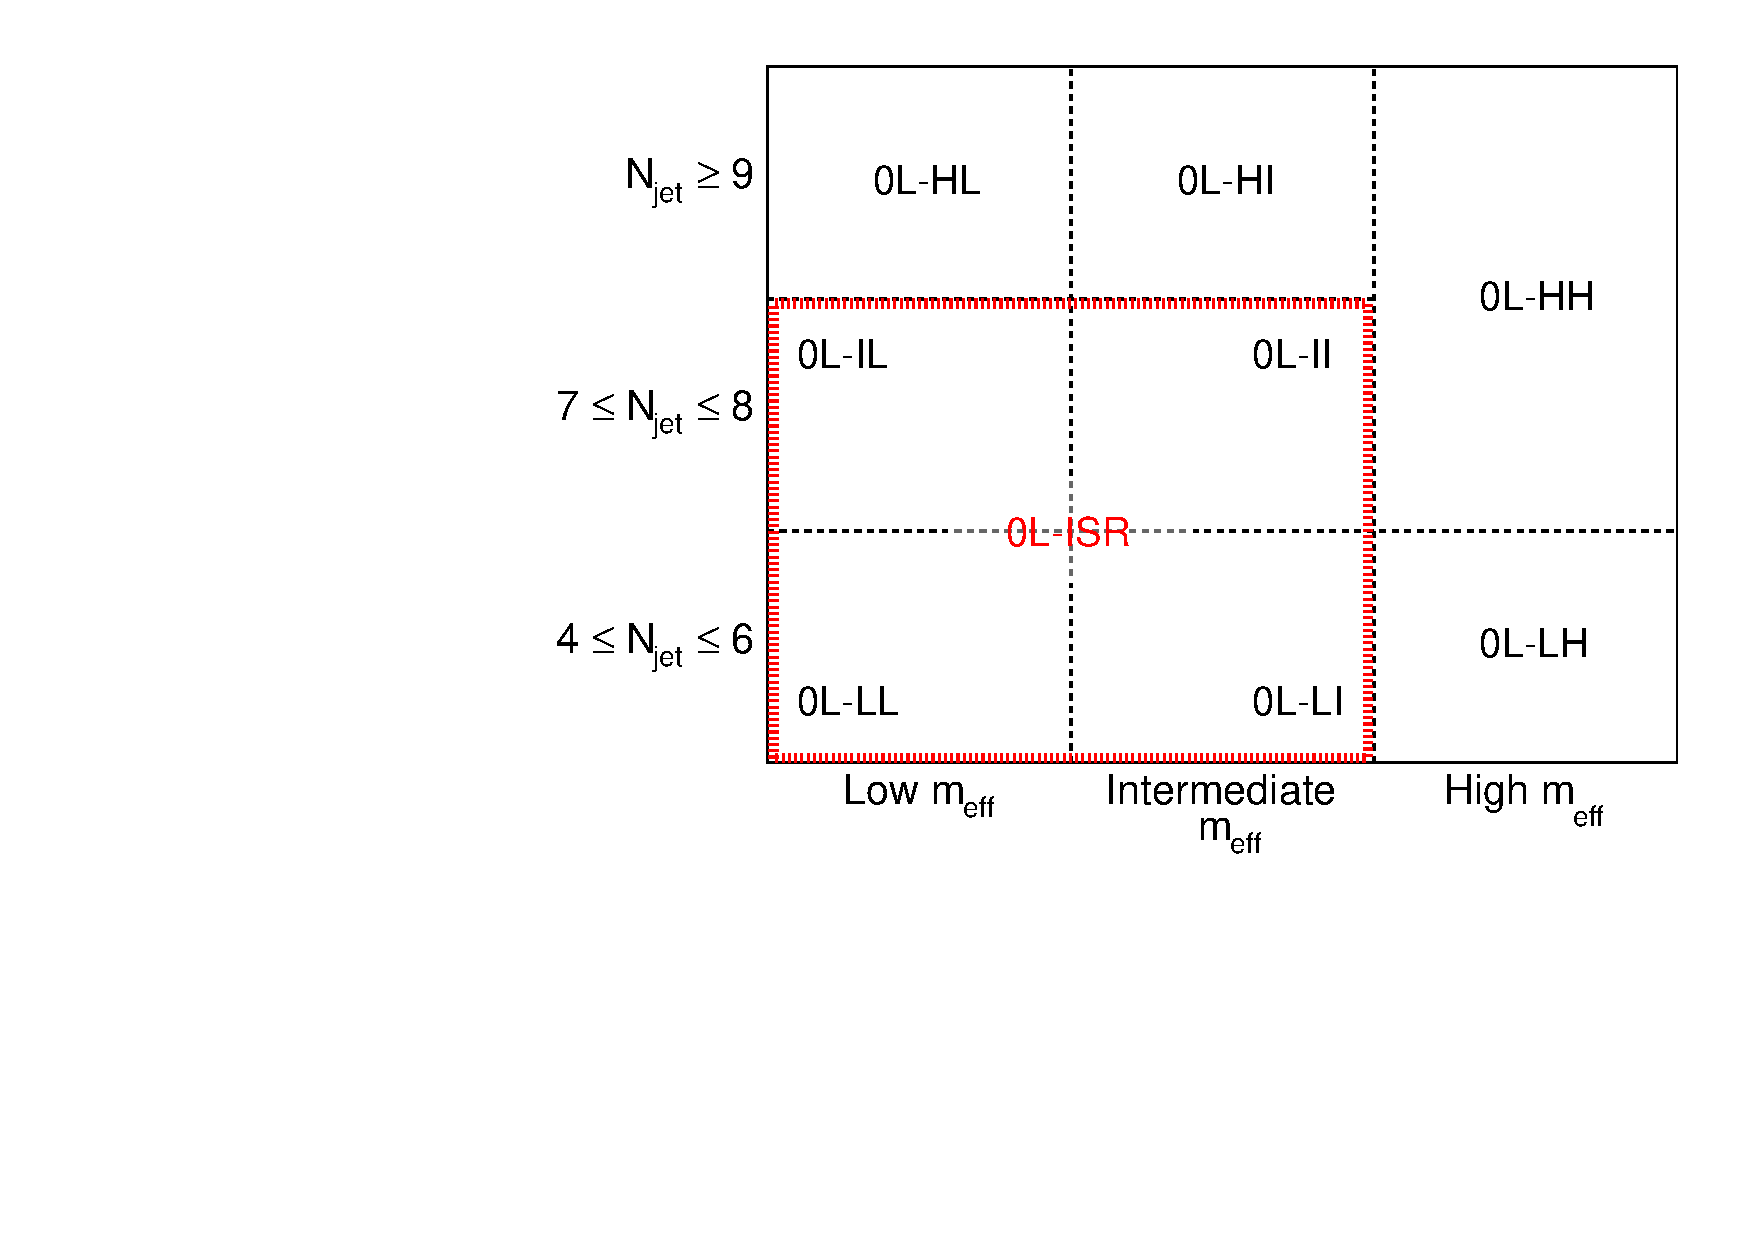
\includegraphics[width=0.49\linewidth]{figures/strong_prod/paper/selections/selections_0lep.pdf}\label{fig:multibin_scheme_0l}}
	\subfigure[]{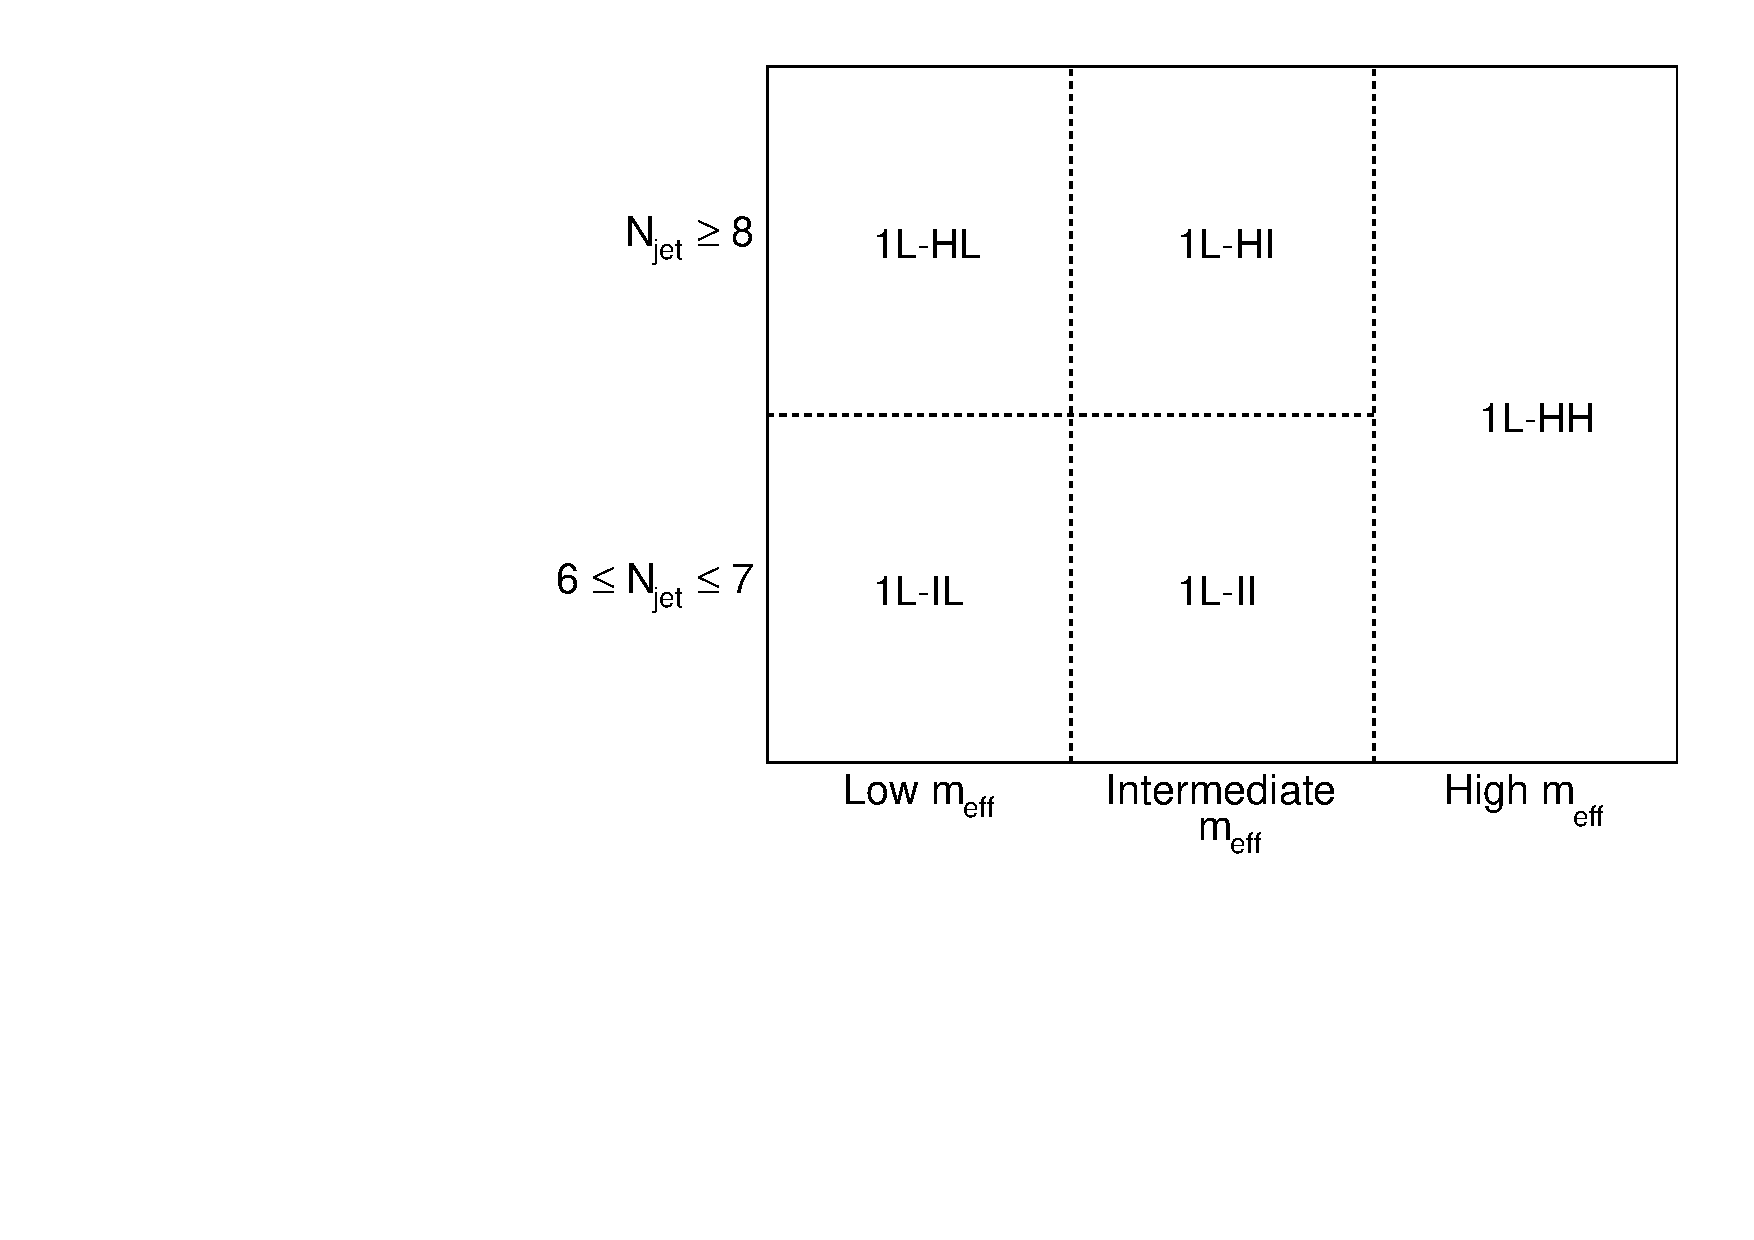
\includegraphics[width=0.49\linewidth]{figures/strong_prod/paper/selections/selections_1lep.pdf}\label{fig:multibin_scheme_1l}}
	\caption{Scheme of the multi-bin analysis for the \subref{fig:multibin_scheme_0l} 0-lepton 
	and \subref{fig:multibin_scheme_1l} 1-lepton regions. 
        The 0L-ISR region is represented with the broad red 
	dashed line in \subref{fig:multibin_scheme_0l}. 
      }
	\label{fig:multibin_scheme}
\end{figure}

\clearpage

\begin{landscape}
	\begin{table}[t]
   		\centering
        		\renewcommand{\arraystretch}{1.5}
                        \caption{Definition of the high-$\njet$ SRs, CRs and VRs of the multi-bin analysis. All kinematic variables are
                          expressed in \gev\ except $\dphimin$, which is in radians.}
                        \label{tab:multibin_Hn}
        		\begin{tabular}{c c c c c c c c c c}
        			\toprule
			\multicolumn{10}{c}{\textbf{ High-$\njet$ regions}}\\
			\multicolumn{10}{c}{Criteria common to all regions: $\nbjet \geq 3$, ${\pt}^\mathrm{jet} > 30$~GeV } \\
			\midrule 
			Targeted kinematics  & Type & \nlep & $\dphimin$ & $\mt$ & \njet & $\mtb$ & $\mjsum$ & $\met$ & $\meff$  \\
			\midrule
			\multirow{5}{*}{\begin{minipage}{3cm}\centering High-\meff\ \\ (HH) \\ (Large \msplit) \end{minipage}} 
			& SR-0L 	& $= 0$  		& $>0.4$ 		& $-$ 		& $\ge 7$		& $>100 $ 			& $>200$ 	& $> 400 $ 				& $> 2500$ \\ 
			& SR-1L 	& $\ge 1$  	& $-$		& $> 150 $ 	& $\ge 6$		& $> 120$ 			& $>200$ 	& $> 500 $ 				& $> 2300$ \\ 
			& CR 	& $\ge 1$  	& $-$ 		& $< 150$ 	& $\ge 6$		& $> 60 $ 				& $>150$ 	& $> 300 $ 				& $> 2100$ \\ 
			& VR-0L 	& $= 0$  		& $>0.4$ 		& $-$ 		& $\ge 7$		& $<100$ if $\met>300$ 	& $-$ 	& $< 300 $ if $\mtb > 100$ 	& $> 2100$ \\
			& VR-1L 	& $\ge 1$  	& $-$ 		& $> 150$ 	& $\ge 6$		& $<140$ if $\meff>2300$	& $-$ 	& $< 500$  				& $> 2100$ \\
			\midrule
			\multirow{5}{*}{\begin{minipage}{3cm}\centering Intermediate-\meff\ \\ (HI) \\ (Intermediate \msplit) \end{minipage}} 
			& SR-0L 	& $= 0$  		& $>0.4$ 		& $-$ 		& $\ge 9$		& $> 140$ 			& $>150$ 	& $> 300 $ 				& $[1800, 2500]$ \\ 
			& SR-1L 	& $\ge 1$  	& $-$		& $> 150 $ 	& $\ge 8$		& $> 140$ 			& $>150$ 	& $> 300 $ 				& $[1800, 2300]$ \\ 
			& CR 	& $\ge 1$  	& $-$ 		& $< 150$ 	& $\ge 8$		& $> 60$ 				& $>150$ 	& $> 200 $ 				& $[1700, 2100]$ \\ 
			& VR-0L 	& $= 0$  		& $>0.4$ 		& $-$ 		& $\ge 9$		& $<140$ if $\met>300$ 	& $-$ 	& $< 300 $ if $\mtb > 140$ 	& $[1650, 2100]$ \\
			& VR-1L 	& $\ge 1$  	& $-$ 		& $> 150$ 	& $\ge 8$		& $<140$ if $\met>300$	& $-$ 	& $< 300 $ if $\mtb > 140$	& $[1600, 2100]$ \\
			\midrule
			\multirow{5}{*}{\begin{minipage}{3cm}\centering Low-\meff\ \\ (HL) \\ (Small \msplit) \end{minipage}} 
			& SR-0L 	& $= 0$  		& $>0.4$ 		& $-$ 		& $\ge 9$		& $> 140$ 			& $-$ 	& $> 300 $ 				& $[900, 1800]$ \\ 
			& SR-1L 	& $\ge 1$  	& $-$		& $> 150 $ 	& $\ge 8$		& $> 140$ 			& $-$ 	& $> 300 $ 				& $[900, 1800]$ \\ 
			& CR 	& $\ge 1$  	& $-$ 		& $< 150$ 	& $\ge 8$		& $> 130$ 			& $-$ 	& $> 250 $ 				& $[900, 1700]$ \\ 
			& VR-0L 	& $= 0$  		& $>0.4$ 		& $-$ 		& $\ge 9$		& $<140$				& $-$ 	& $> 300 $ 				& $[900, 1650]$ \\
			& VR-1L 	& $\ge 1$  	& $-$ 		& $> 150$ 	& $\ge 8$		& $<140$				& $-$ 	& $> 225 $			 	& $[900, 1650]$ \\
      			\bottomrule
    		\end{tabular}
 	\end{table}
\end{landscape}

\clearpage

\begin{landscape}
	\begin{table}[t]
		\small
   		\centering
        		\renewcommand{\arraystretch}{1.5}
                        \caption{Definition of the intermediate-$\njet$ SRs, CRs and VRs of the multi-bin analysis. All kinematic variables are
                          expressed in \gev\ except $\dphimin$, which is in radians. The $\leadjet = b$  requirement specifies that 
                          the leading jet is $b$-tagged.}
                        \label{tab:multibin_In}
        		\begin{tabular}{c c c c c c c c c c c}
        			\toprule
			\multicolumn{11}{c}{\textbf{ Intermediate-$\njet$ regions}}\\
			\multicolumn{11}{c}{Criteria common to all regions: $\nbjet \geq 3$, ${\pt}^\mathrm{jet} > 30$~GeV } \\
			\midrule 
			Targeted kinematics  & Type & $N_\mathrm{lepton}$ & $\dphimin$ & $\mt$ & $\njet$ & $\leadjet = b$ or $\dphilead \leq 2.9$ & $\mtb$ & $\mjsum$  & $\met$ & $\meff$  \\
			\midrule
			\multirow{5}{*}{\begin{minipage}{3cm}\centering Intermediate-\meff\ \\ (II) \\ (Intermediate \msplit) \end{minipage}} 
			& SR-0L 	& $= 0$  		& $>0.4$ 		& $-$ 		& $[7,8]$		& \cmark		& $> 140 $ 			& $>150$ 		& $> 300 $ 				& $[1600,2500]$ \\ 
			& SR-1L 	& $\ge 1$  	& $-$		& $> 150 $ 	& $[6,7]$		& $-$ 		& $> 140$ 			& $>150$ 		& $> 300 $ 				& $[1600,2300]$ \\ 
			& CR 	& $\ge 1$  	& $-$ 		& $< 150$ 	& $[6,7]$		& \cmark 		& $> 110 $ 			& $>150$ 		& $> 200 $ 				& $[1600,2100]$ \\ 
			& VR-0L 	& $= 0$  		& $>0.4$ 		& $-$ 		& $[7,8]$		& \cmark		& $<140$ 				& $-$ 		& $> 300 $ 				& $[1450,2000]$ \\
			& VR-1L 	& $\ge 1$  	& $-$ 		& $> 150$ 	& $[6,7]$		& $-$		& $<140$				& $-$ 		& $> 225 $  				& $[1450,2000]$ \\
			\midrule
			\multirow{5}{*}{\begin{minipage}{3cm}\centering Low-\meff\ \\ (IL) \\ (Low \msplit) \end{minipage}} 
			& SR-0L 	& $= 0$  		& $>0.4$ 		& $-$ 		& $[7,8]$		& \cmark		& $> 140 $ 			& $-$ 		& $> 300 $ 				& $[800,1600]$ \\ 
			& SR-1L 	& $\ge 1$  	& $-$		& $> 150 $ 	& $[6,7]$		& $-$ 		& $> 140$ 			& $-$ 		& $> 300 $ 				& $[800,1600]$ \\ 
			& CR 	& $\ge 1$  	& $-$ 		& $< 150$ 	& $[6,7]$		& \cmark 		& $> 130 $ 			& $-$ 		& $> 300 $ 				& $[800,1600]$ \\ 
			& VR-0L 	& $= 0$  		& $>0.4$ 		& $-$ 		& $[7,8]$		& \cmark		& $<140$ 				& $-$ 		& $> 300 $ 				& $[800,1450]$ \\
			& VR-1L 	& $\ge 1$  	& $-$ 		& $> 150$ 	& $[6,7]$		& $-$		& $<140$				& $-$ 		& $> 300 $  				& $[800,1450]$ \\
      			\bottomrule
    		\end{tabular}
 	\end{table}
\end{landscape}

\clearpage

\begin{landscape}
	\begin{table}[t]
   		\centering
        		\renewcommand{\arraystretch}{1.1}
                        \caption{Definition of the low-$\njet$ and ISR SRs, CRs and VRs of the multi-bin analysis. All kinematic variables are
                          expressed in \gev\ except $\dphimin$, which is
                          in radians. The $\leadjet = b$ ($\leadjet \neq b$) requirement specifies that 
                          the leading jet is (not) $b$-tagged.}
                        \label{tab:multibin_Ln}
                        \label{tab:multibin_ISR}		
        		\begin{tabular}{c c c c c c c c c c c }
        			\toprule
			\multicolumn{11}{c}{\textbf{ Low-$\njet$ regions}}\\
			\multicolumn{11}{c}{Criteria common to all regions: $\nbjet \geq 3$, ${\pt}^\mathrm{jet} > 30$~GeV } \\
			\midrule 
			Targeted kinematics  & Type & $N_\mathrm{lepton}$ & $\dphimin$ & $\mt$ & $\njet$ & $\leadjet = b$ or $\dphilead \leq 2.9$ & $\pt^{\fourthjet}$ & $\mtb$ & $\met$ & $\meff$  \\
			\midrule
			\multirow{3}{*}{\begin{minipage}{3cm}\centering High-\meff\ \\ (LH) \\ (Large \msplit) \end{minipage}} 
			& SR 	& $= 0$  		& $>0.4$ 		& $-$ 		& $[4,6]$		& $-$		& $>90$					& $-$ 			& $> 300 $ 				& $> 2400$ \\ 
			& CR 	& $\ge 1$  	& $-$ 		& $< 150$ 	& $[4,5]$		& $-$ 	 	& -						& $-$ 			& $> 200 $ 				& $> 2100$ \\ 
			& VR 	& $= 0$  		& $>0.4$ 		& $-$ 		& $[4,6]$		& $-$ 		& $>90$ if $\met < 300$		& $-$			& $> 200 $ 				& $[2000,2400]$ \\
			\midrule
			\multirow{3}{*}{\begin{minipage}{3cm}\centering Intermediate-\meff\ \\ (LI) \\ (Intermediate \msplit) \end{minipage}} 
			& SR 	& $= 0$  		& $>0.4$ 		& $-$ 		& $[4,6]$		& \cmark		& $>90$				& $>140$ 		& $> 350 $ 				& $[1400,2400]$ \\ 
			& CR 	& $\ge 1$  	& $-$ 		& $< 150$ 	& $[4,5]$		& \cmark 	 	& $>70$				& $-$ 		& $> 300 $ 				& $[1400,2000]$ \\ 
			& VR 	& $= 0$  		& $>0.4$ 		& $-$ 		& $[4,6]$		& \cmark		& $>90$				& $<140$ 		& $> 300 $ 				& $[1250,1800]$ \\
			\midrule
			\multirow{3}{*}{\begin{minipage}{3cm}\centering Low-\meff\ \\ (LL) \\ (Low \msplit) \end{minipage}} 
			& SR 	& $= 0$  		& $>0.4$ 		& $-$ 		& $[4,6]$		& \cmark		& $>90$				& $>140$ 		& $> 350 $ 				& $[800,1400]$ \\ 
			& CR 	& $\ge 1$  	& $-$ 		& $< 150$ 	& $[4,5]$		& \cmark 	 	& $>70$				& $-$ 		& $> 300 $ 				& $[800,1400]$ \\ 
			& VR 	& $= 0$  		& $>0.4$ 		& $-$ 		& $[4,6]$		& \cmark		& $>90$				& $<140$ 		& $> 300 $ 				& $[800,1250]$ \\
      			\bottomrule
    		\end{tabular}
		
		\par\medskip
		
    		\begin{tabular}{K{1.5cm} K{1.5cm} K{1.5cm} K{1.5cm} K{1.5cm} K{1.5cm} K{1.5cm} K{1.5cm} }
        			\toprule
			\multicolumn{8}{c}{\textbf{ ISR regions}}\\
			\multicolumn{8}{c}{Criteria common to all regions: $\nbjet \geq 3$, $\dphilead > 2.9$, ${\pt}^\leadjet > 400$~\gev, ${\pt}^\mathrm{jet} > 30$~GeV, $\leadjet \neq b$} \\
			\midrule 
			Type & $N_\mathrm{lepton}$ & $\dphimin$ & $\mt$ & $\njet$ & $\mtb$ & $\met$ & $\meff$  \\
			\midrule
			SR 	& $= 0$  		& $>0.4$ 		& $-$ 		& $[4,8]$		& $>100$ 			& $> 600 $ 				& $<2200$ \\ 
			CR 	& $\ge 1$  	& $-$ 		& $< 150$ 	& $[4,7]$		& $-$ 			& $> 400 $ 				& $<2000$ \\ 
			VR 	& $= 0$  		& $>0.4$ 		& $-$ 		& $[4,8]$		& $>100$ 			& $> 250 $ 				& $<2000$ \\
      			\bottomrule
    		\end{tabular}
 	\end{table}
\end{landscape}

\clearpage 

\section{Systematic uncertainties}
\label{sec:strong:syst}

\begin{figure}[htbp]
	\centering
	\subfigure[]{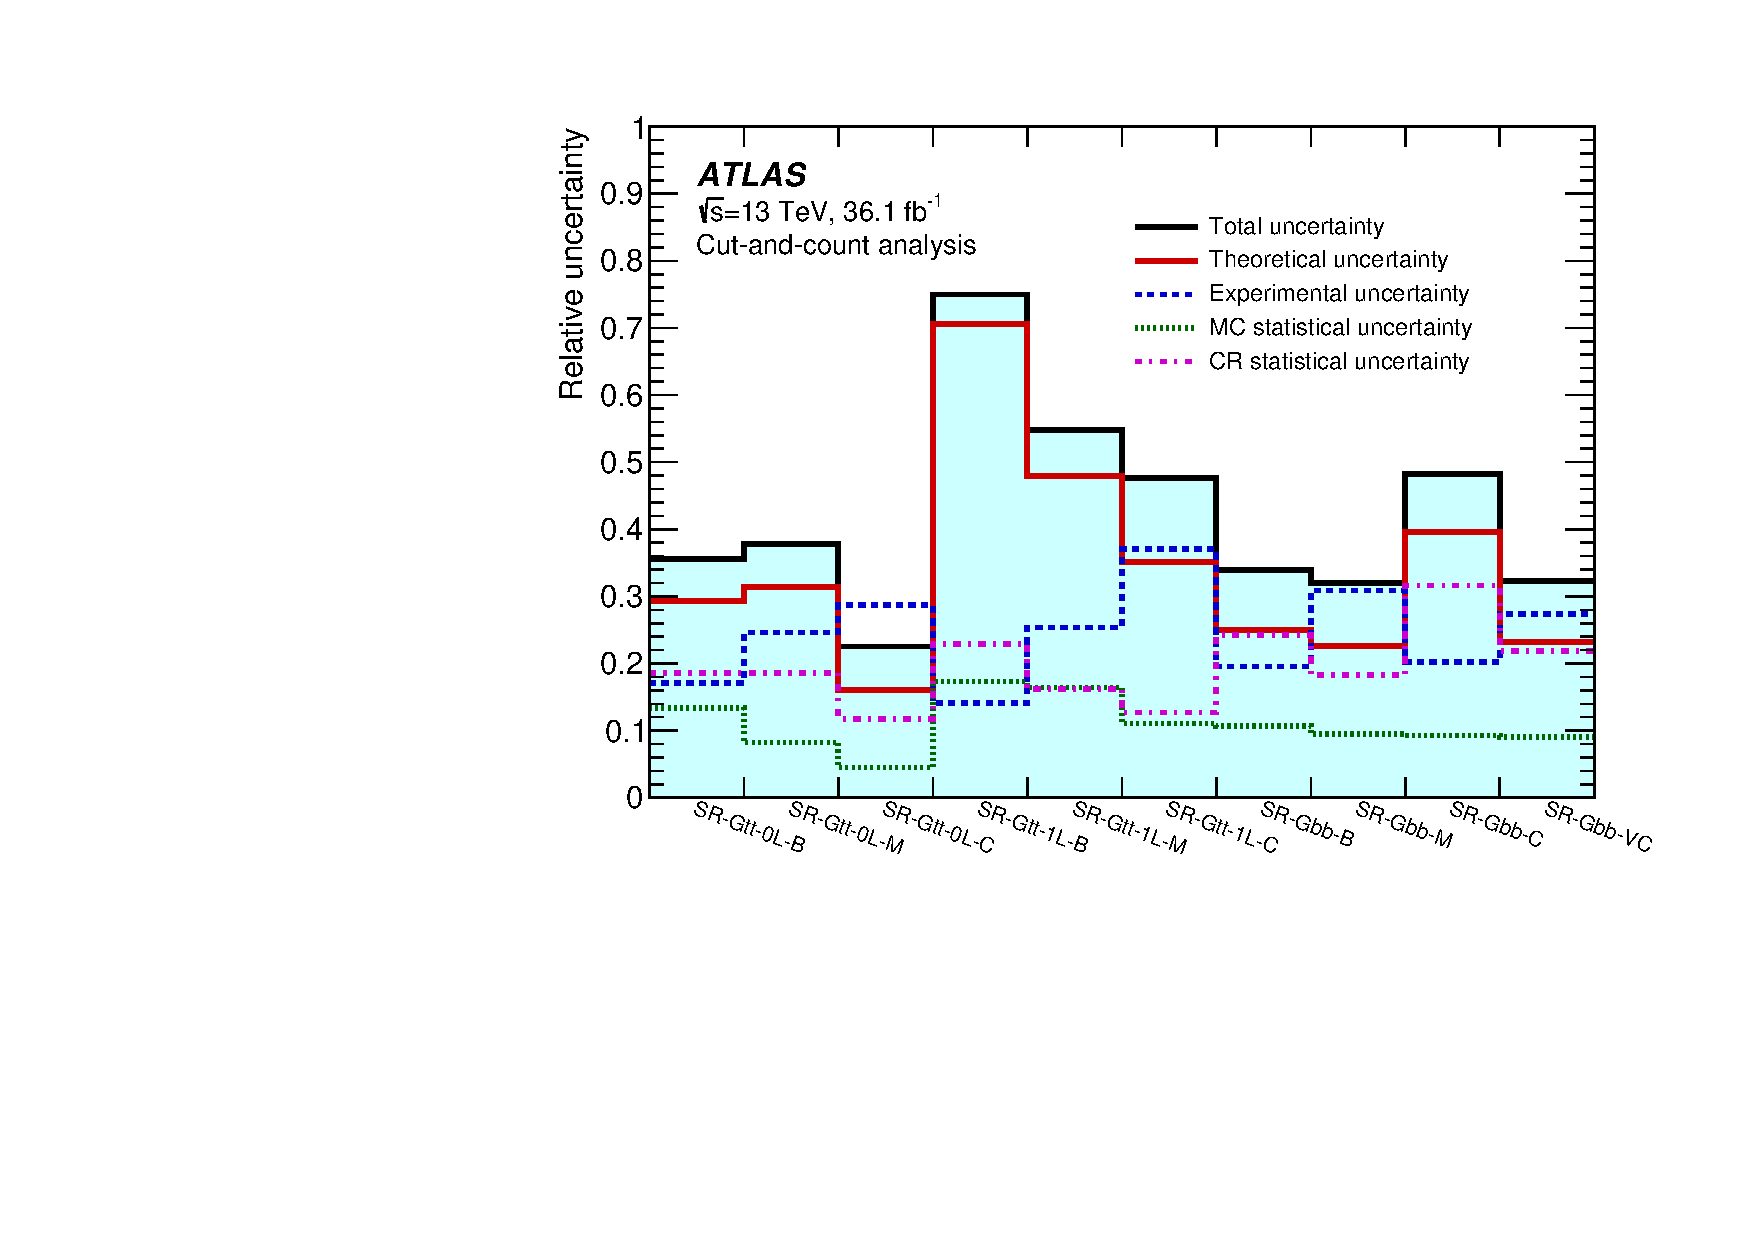
\includegraphics[width=0.85\textwidth]{figures/strong_prod/paper/Cut_and_Count.pdf}\label{fig:syst_cutandcount}}\\
	\subfigure[]{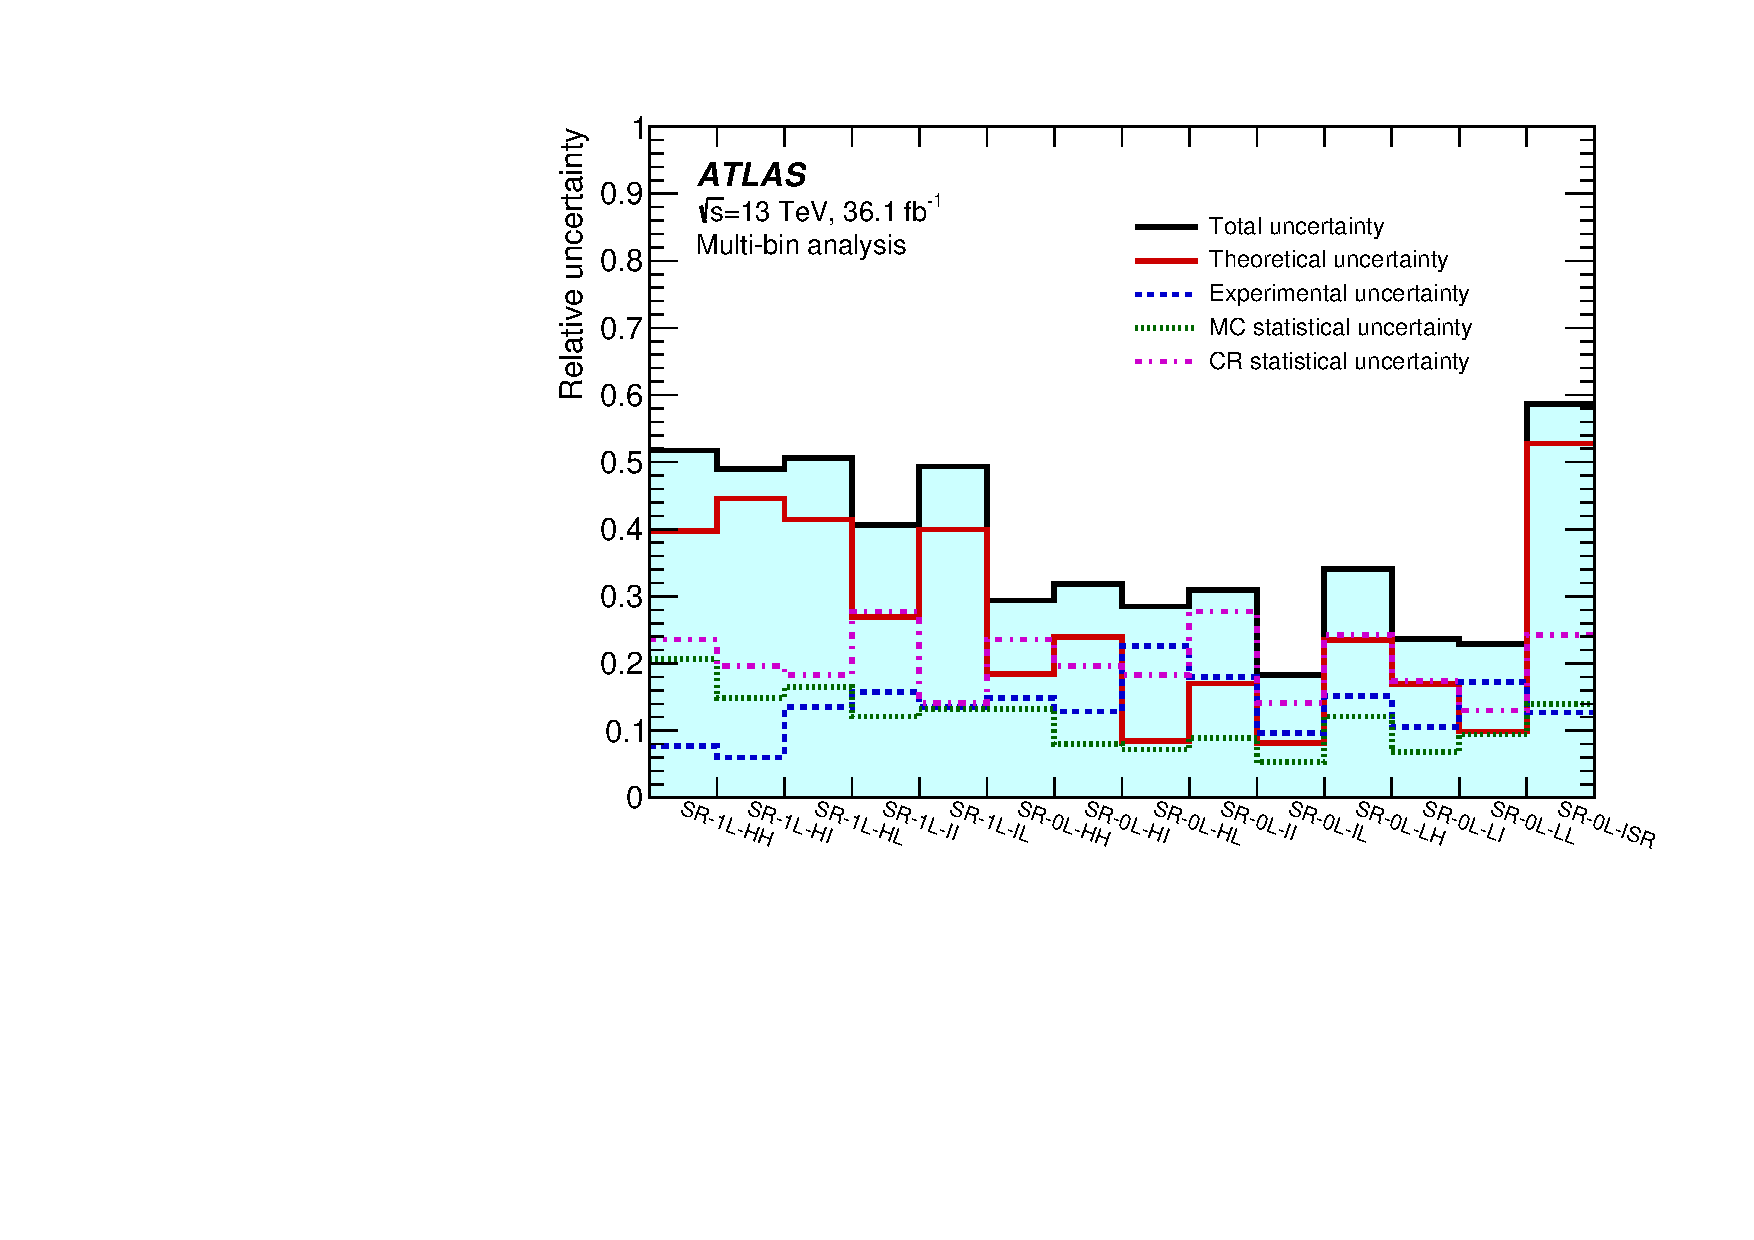
\includegraphics[width=0.85\textwidth]{figures/strong_prod/paper/Multi_bin.pdf}\label{fig:syst_multibin}}\\
	\caption{Relative systematic uncertainty in the background estimate for the \subref{fig:syst_cutandcount} cut-and-count and \subref{fig:syst_multibin} multi-bin analyses. The individual uncertainties can be correlated, such that the total background uncertainty is not necessarily their sum in quadrature.
	} 
	\label{fig:syst}
\end{figure}

\section{Results}

\begin{figure}[htbp]
	\centering
	\subfigure[]{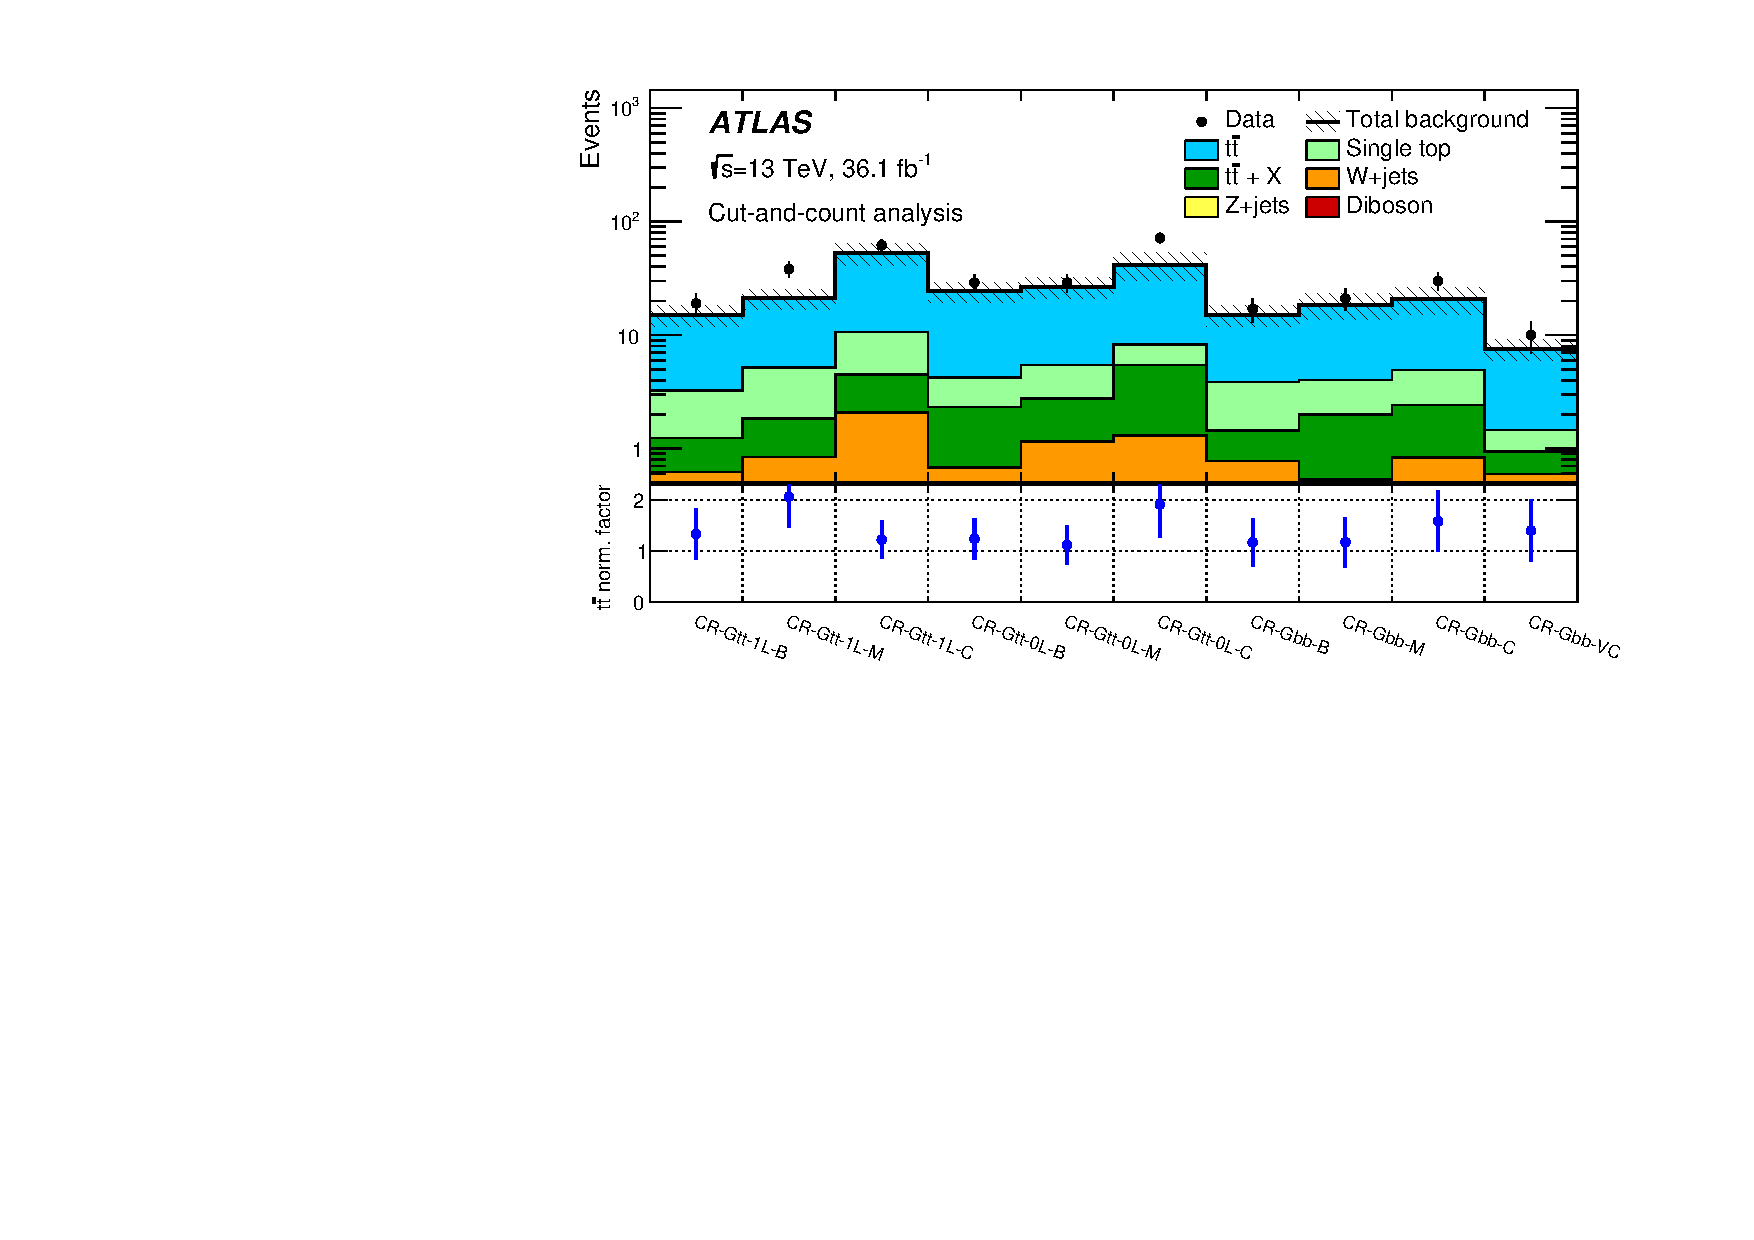
\includegraphics[width=0.9\textwidth]{figures/strong_prod/paper/pulls/histpull_pulls_in_CRs_17_06_23_singlebin.pdf}\label{fig:pullCR_discovery}}
	\subfigure[]{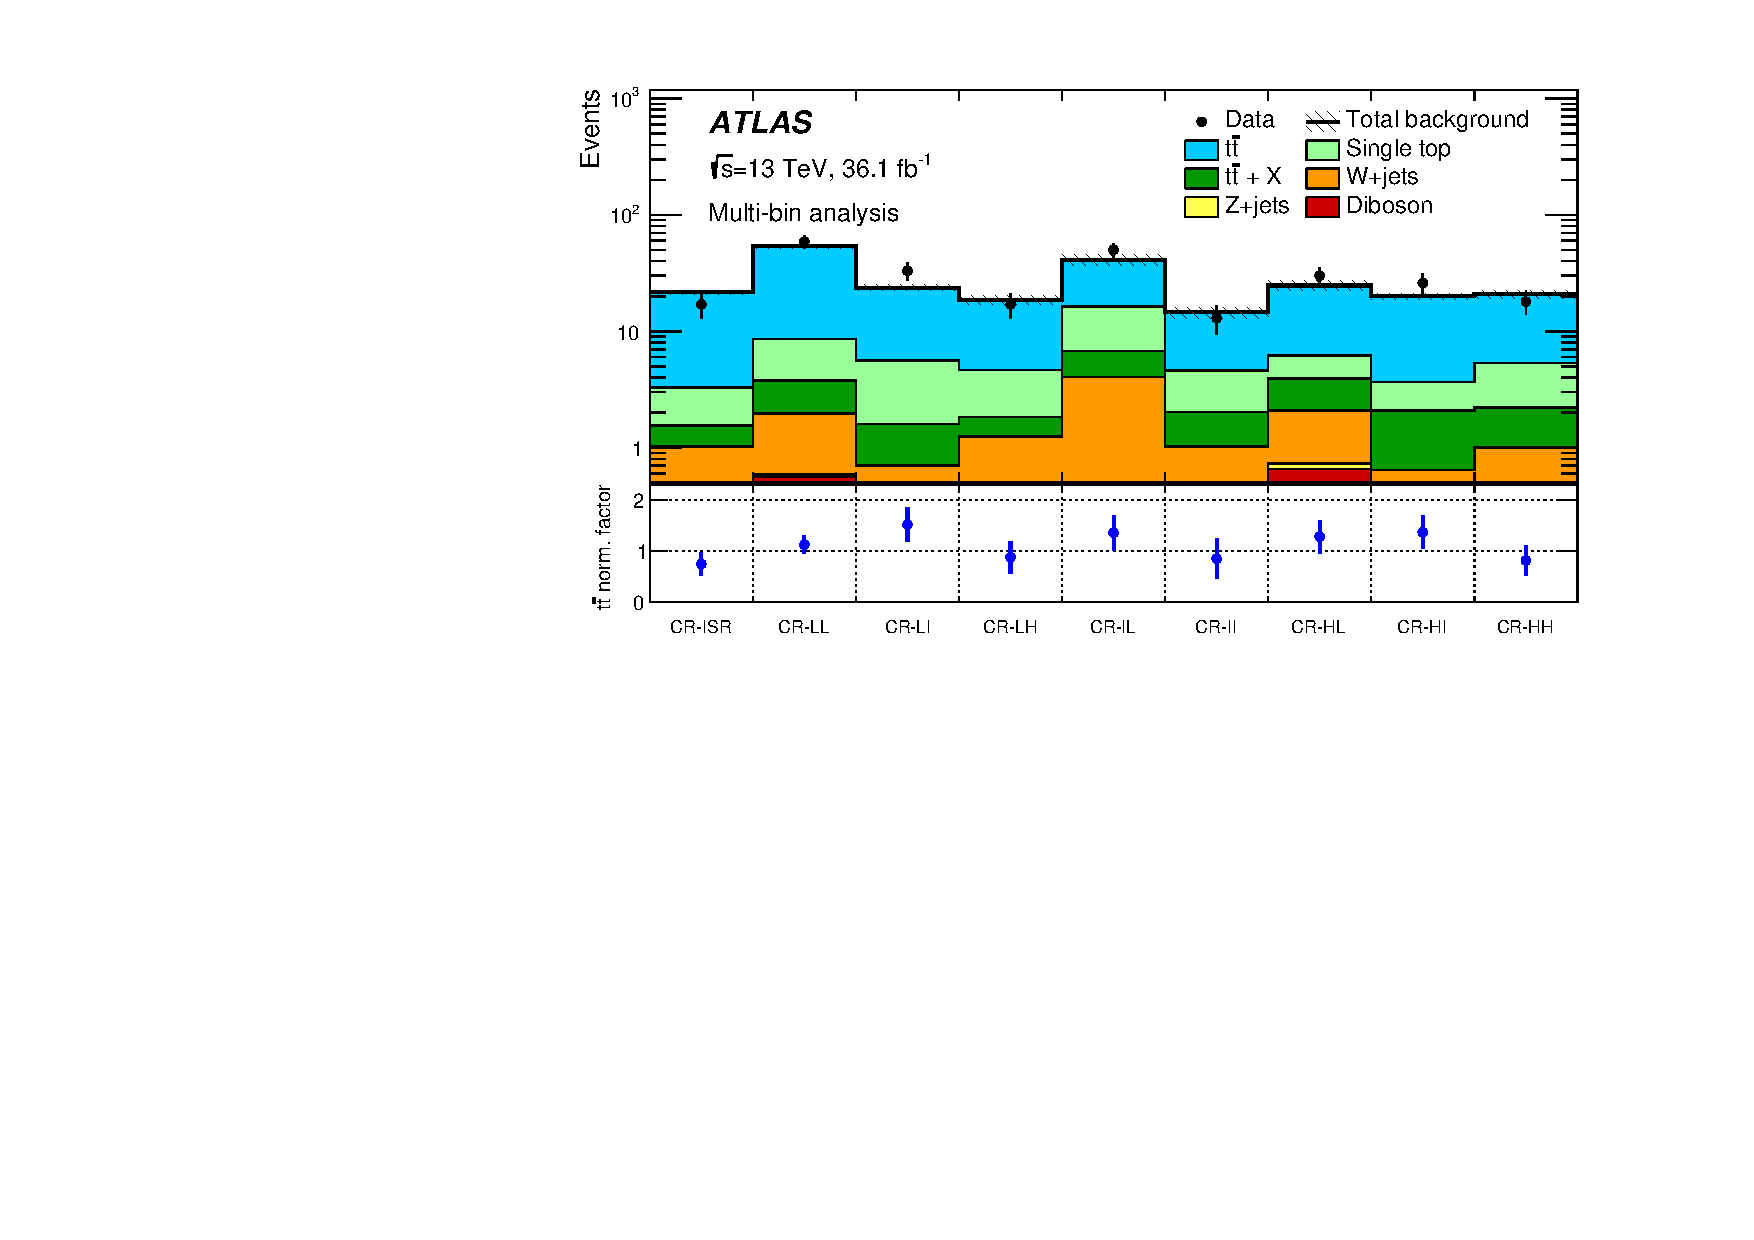
\includegraphics[width=0.9\textwidth]{figures/strong_prod/paper/pulls/histpull_pulls_in_CRs_multichannel_17_06_23.pdf}\label{fig:pullCR_exclusion}}
	\caption{Pre-fit event yield in control regions and related \ttbar
          normalization factors after the background-only fit for
          \subref{fig:pullCR_discovery} 
		the cut-and-count and \subref{fig:pullCR_exclusion} the multi-bin analyses. The upper panel shows 
		the observed number of events and the predicted background yield before the fit.
		The background category \ttbar+X includes \ttbar+W/Z, \ttbar+H and \ttbar\ttbar events. All of these
                regions require at least one signal lepton, for which the
                multijet background is negligible. All uncertainties describes in Section \ref{sec:strong:syst} are included in the uncertainty band.
		The \ttbar normalisation is obtained from the fit
                and is displayed in the bottom panel. 
	} 
	\label{fig:pullCR}
\end{figure}


\begin{figure}[htbp]
	\centering
	\subfigure[]{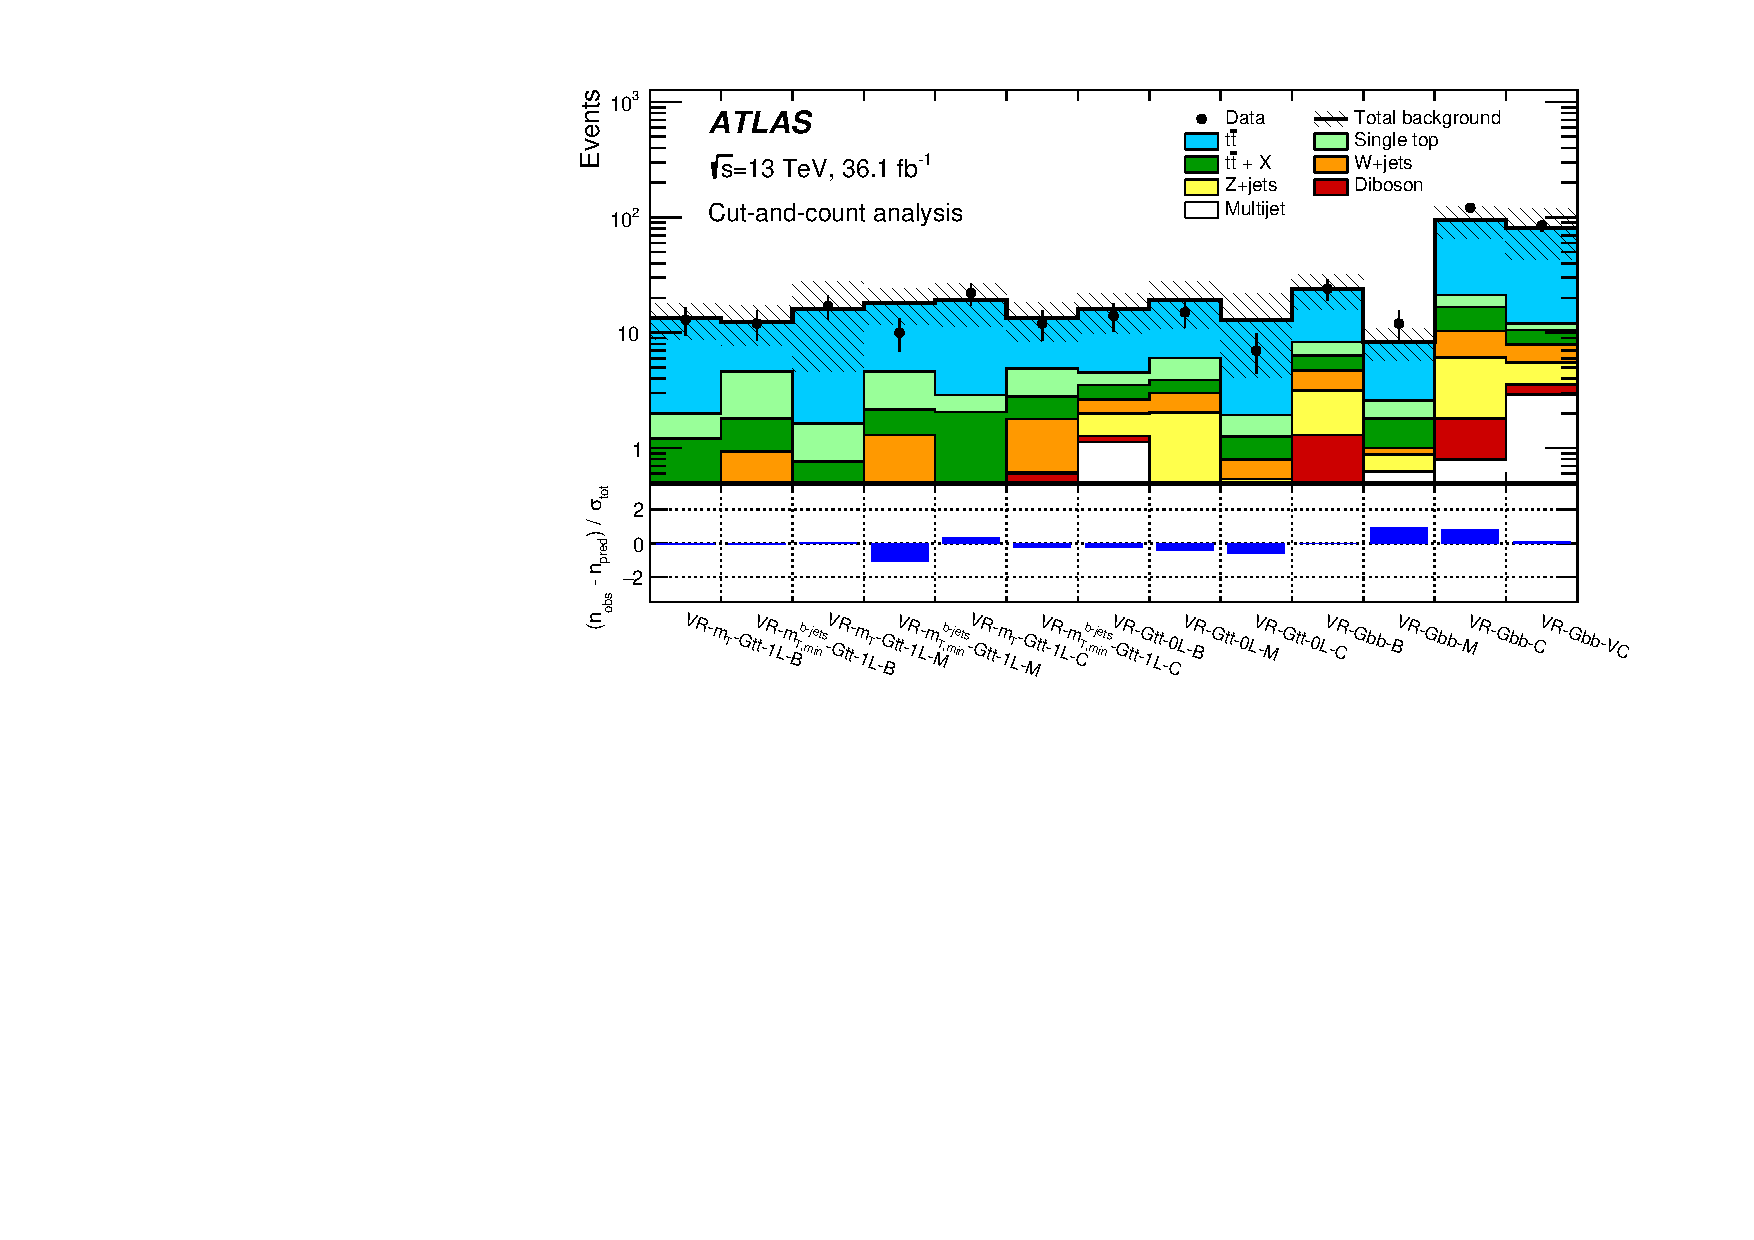
\includegraphics[width=0.9\textwidth]{figures/strong_prod/paper/pulls/histpull_pulls_in_VRs_17_06_23_singlebin.pdf}\label{fig:pullVR_discovery}}\\
	\subfigure[]{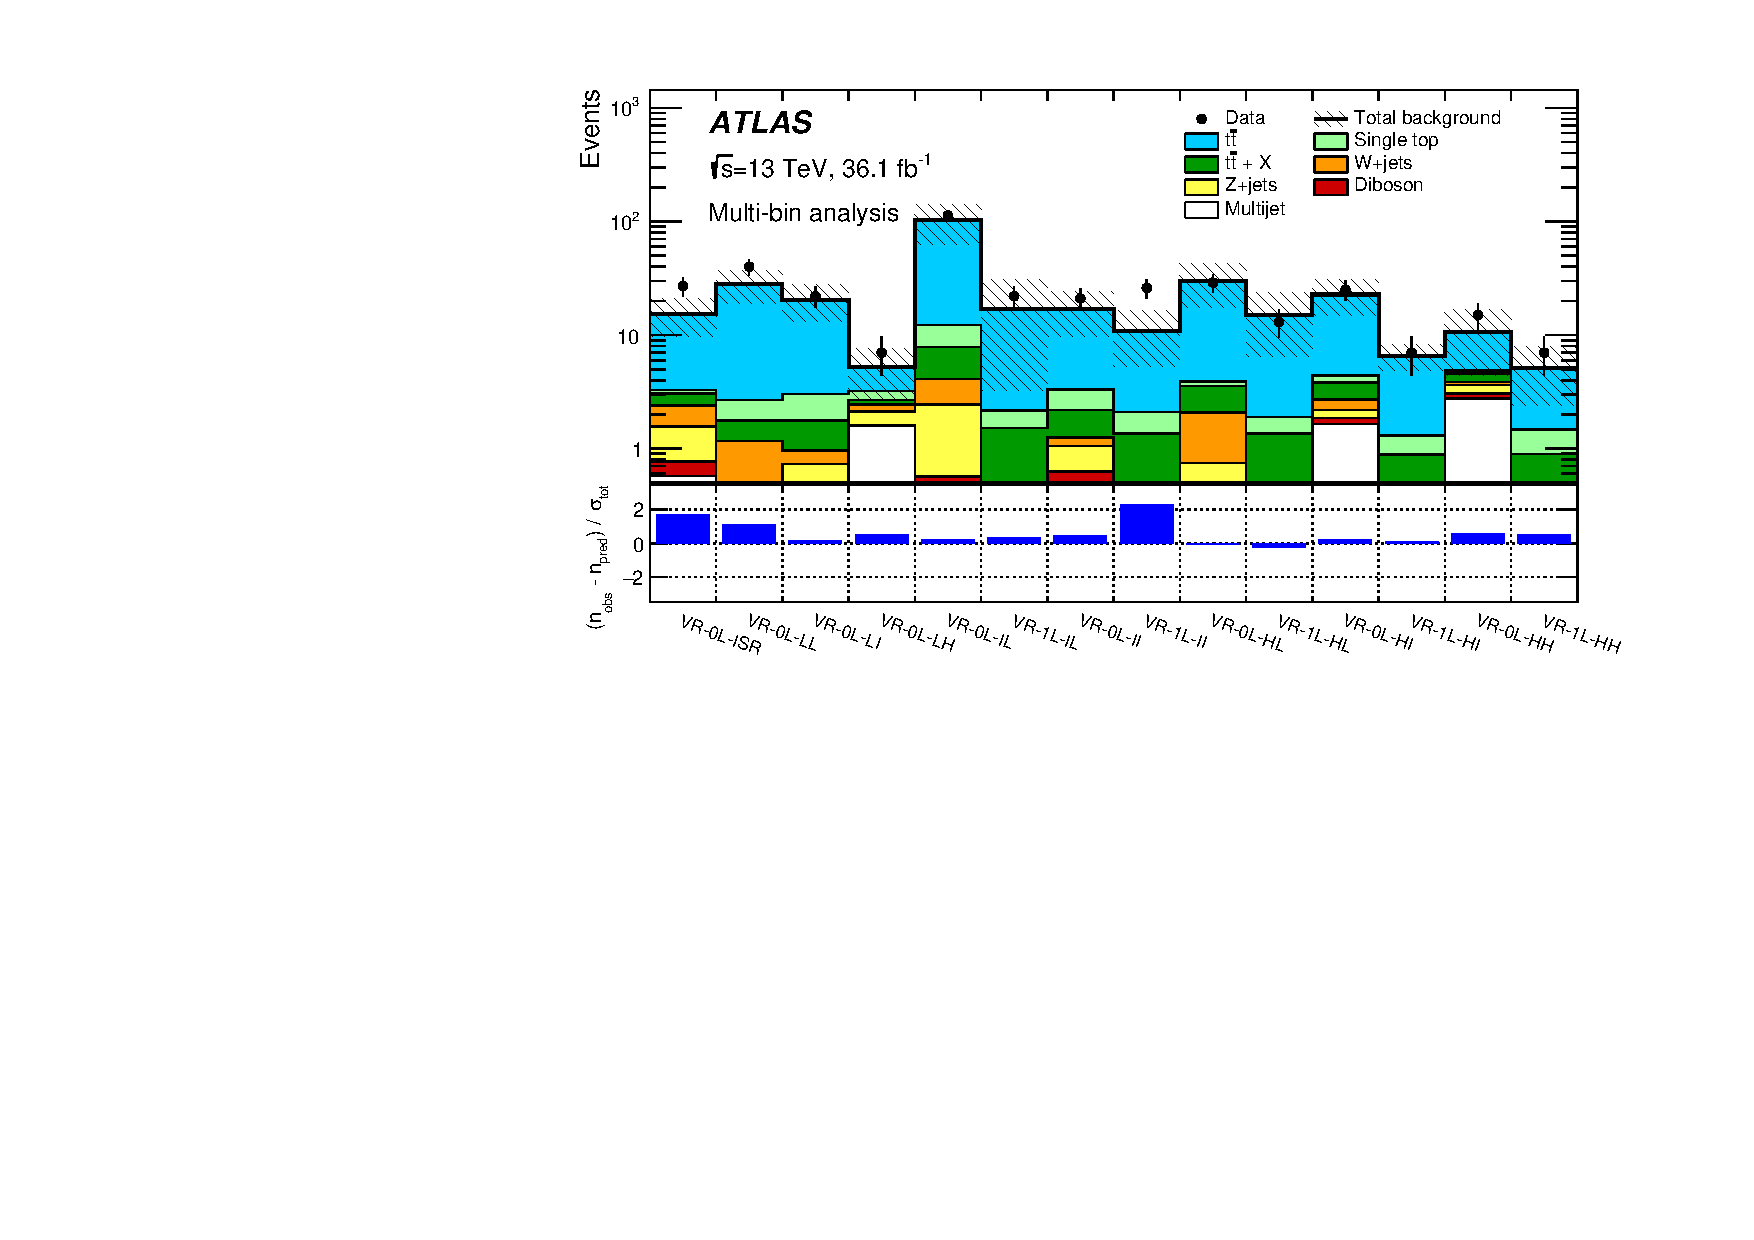
\includegraphics[width=0.9\textwidth]{figures/strong_prod/paper/pulls/histpull_pulls_in_VRs_multichannel_17_06_23.pdf}\label{fig:pullVR_exclusion}}\\
	\caption{Results of the background-only fit extrapolated to the VRs of \subref{fig:pullVR_discovery} the cut-and-count and \subref{fig:pullVR_exclusion}
		the multi-bin analyses. The \ttbar normalisation 
		is obtained from the fit to the CRs shown in Figure~\ref{fig:pullCR}. The upper panel shows 
		the observed number of events and the predicted background yield.
		All uncertainties  defined in Section~\ref{sec:syst} are included in the 
		uncertainty band. The background category \ttbar+X includes \ttbar+W/Z, 
		\ttbar+H and \ttbar\ttbar events. The lower panel shows the pulls in 
		each VR. 
	} 
	\label{fig:pullVR}
\end{figure}


\begin{figure}[htbp]
	\centering
	\subfigure[]{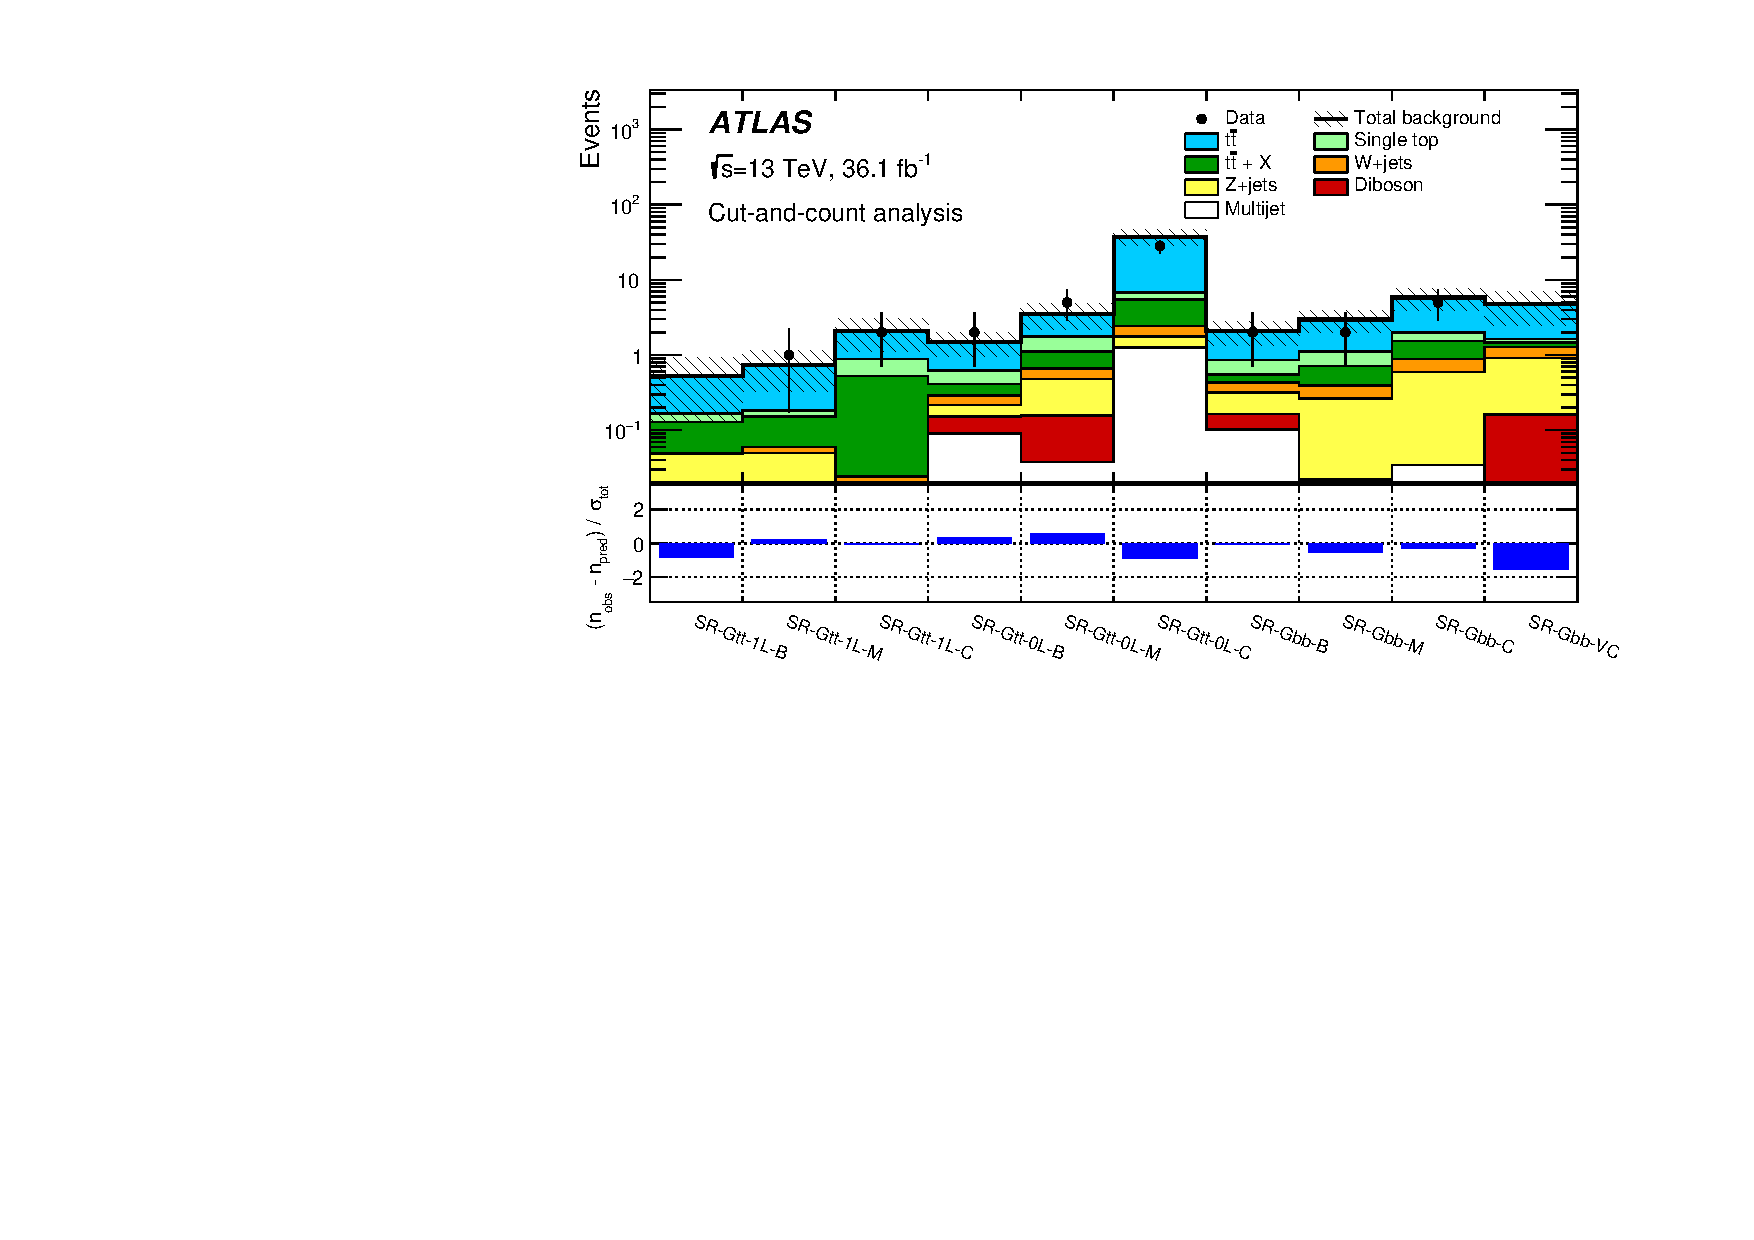
\includegraphics[width=0.9\textwidth]{figures/strong_prod/paper/pulls/histpull_pulls_in_SRs_17_06_23_singlebin.pdf}\label{fig:pullSR_discovery}}\\
	\subfigure[]{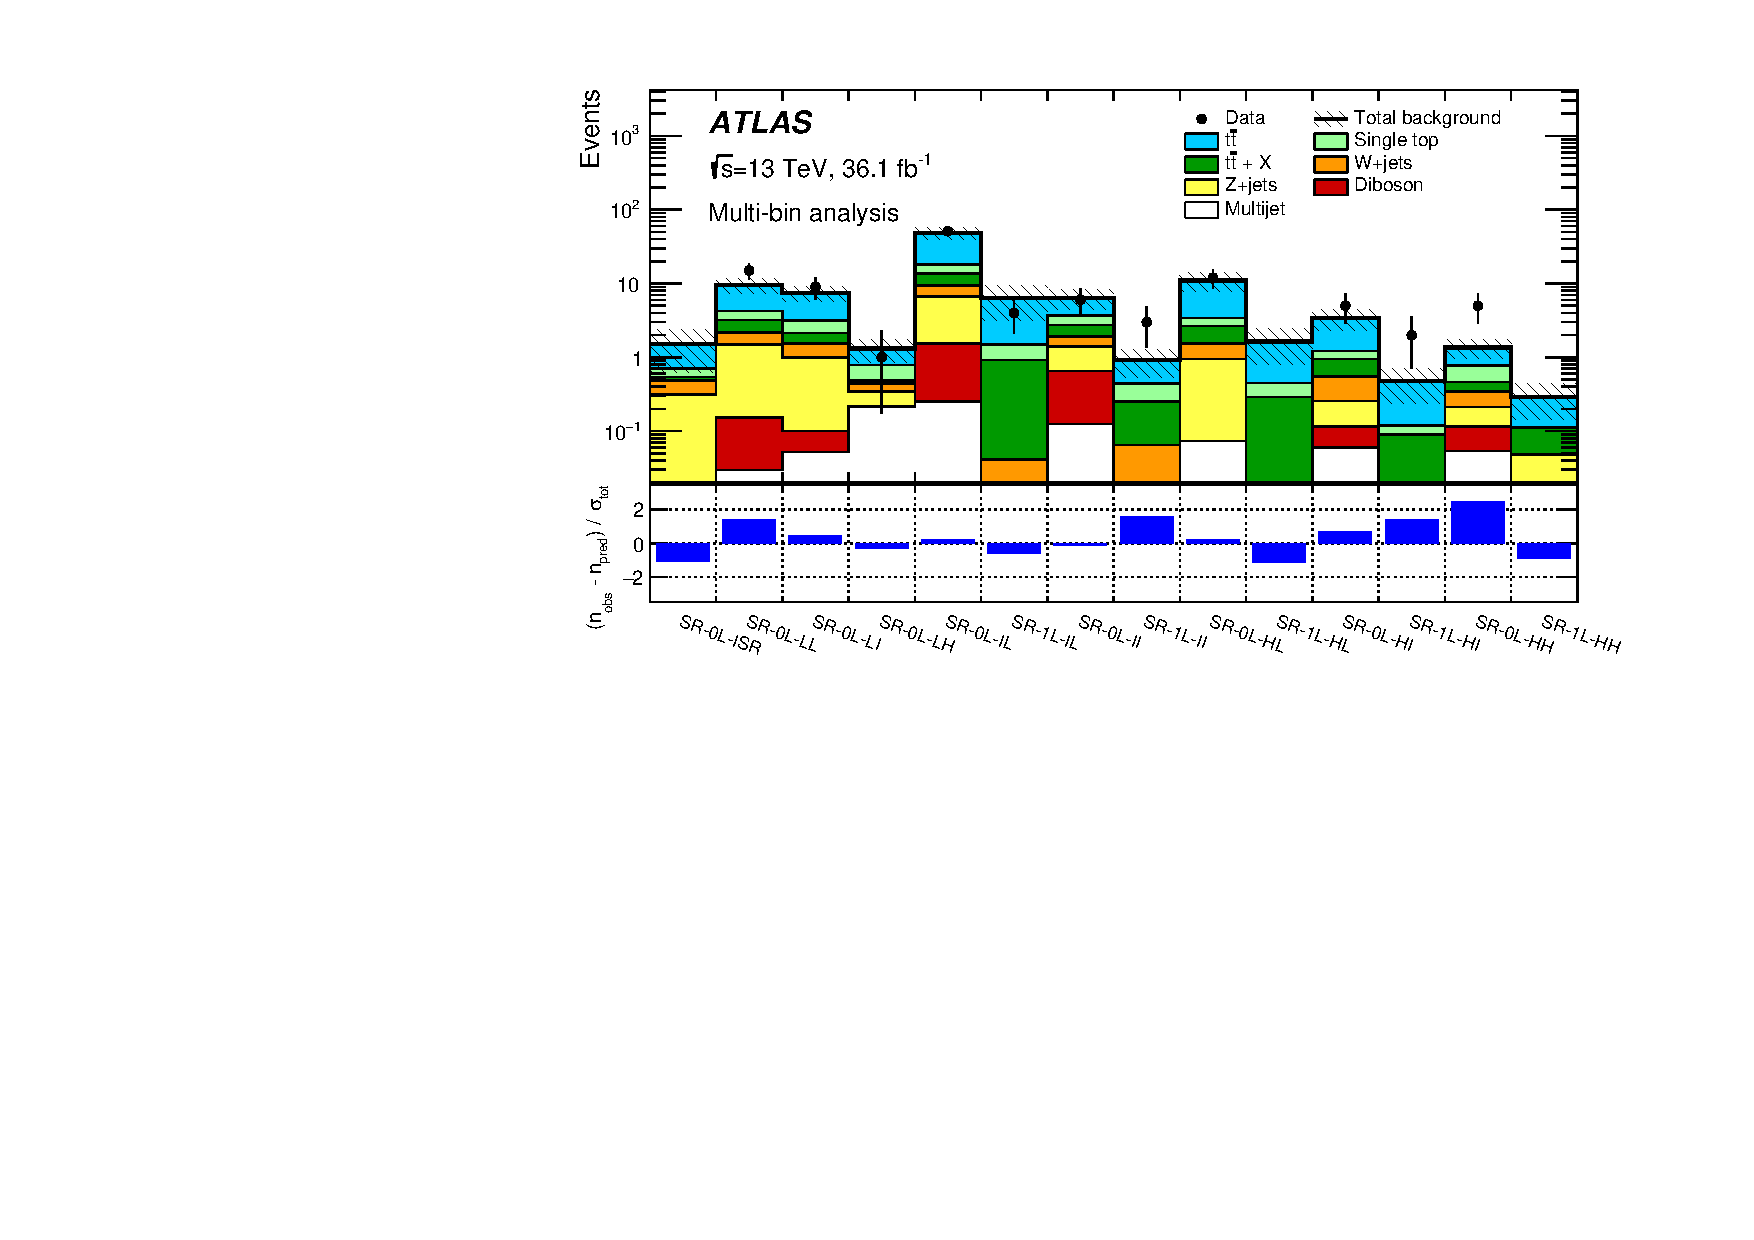
\includegraphics[width=0.9\textwidth]{figures/strong_prod/paper/pulls/histpull_pulls_in_SRs_multichannel_17_06_23.pdf}\label{fig:pullSR_exclusion}}\\
	\caption{Results of the background-only fit extrapolated to the SRs for \subref{fig:pullSR_discovery}
	the cut-and-count and \subref{fig:pullSR_exclusion} the multi-bin analyses. The data in the  SRs are 
	not included in the fit.  The upper panel shows the observed number of events and the predicted background 
	yield. All uncertainties  defined in Section~\ref{sec:syst} are included in the uncertainty band. The background 
	category $\ttbar+X$ includes $\ttbar W/Z$, $\ttbar H$ and $\ttbar \ttbar$ events. The lower panel shows the 
	pulls in each SR.} 
	\label{fig:pullSR}
\end{figure}

\clearpage 

\section{Interpretation}

\subsection{Model-independent limits}

\begin{table}[t]
        \centering
        \caption{The $p_0$-values and $Z$ (the number of equivalent Gaussian standard deviations), 
        	the 95$\%$ CL upper limits on the visible cross-section
                ($\sigma^{95}_\mathrm{vis}$),
                and the observed and
                expected 95$\%$ CL upper limits on the number of BSM events ($S_{\textrm
                obs}^{95}$ and $S_{\textrm exp}^{95}$). The maximum
              allowed $p_0$-value
              is truncated at 0.5.}
        \label{mod-ind-lim}
        \small
        \begin{tabular*}{0.6\textwidth}{@{\extracolsep{\fill}}lcccc}
                \noalign{\smallskip}\toprule\noalign{\smallskip}
                Signal channel         & $p_0$ (Z)            & $\sigma^{95}_\mathrm{vis}$ [fb]  &  $S_{\textrm obs}^{95}$  & $S_{\textrm exp}^{95}$   \\
                \noalign{\smallskip}\midrule \noalign{\smallskip}
                SR-Gtt-1L-B & $ 0.50~(0.00) $ &  $0.08$ &  $3.0$ & $ { 3.0 }^{ +1.0 }_{ -0.0 }$ \\[1mm]
                SR-Gtt-1L-M & $ 0.34~(0.42)$ &  $0.11$ &  $3.9$ & $ { 3.6 }^{ +1.1 }_{ -0.4 }$ \\[1mm]
                SR-Gtt-1L-C & $ 0.50~(0.00)$ &  $0.13$ &  $4.8$ & $ { 4.7 }^{ +1.8 }_{ -0.9 }$ \\[1mm]
                \noalign{\smallskip}\midrule \noalign{\smallskip}
                SR-Gtt-0L-B & $ 0.32~(0.48)$ & $0.13$ &  $4.8$ & $ { 4.1 }^{ +1.7 }_{ -0.6 }$  \\[1mm]
                SR-Gtt-0L-M & $ 0.25~(0.69)$ &  $0.21$ &  $7.5$ & $ { 6.0 }^{ +2.3 }_{ -1.4 }$ \\[1mm]
                SR-Gtt-0L-C & $ 0.50~(0.00)$ &  $0.39$ &  $14.0$ & $ { 17.8 }^{ +6.6 }_{ -4.5 }$ \\[1mm] %%to be updated
                \noalign{\smallskip}\midrule\noalign{\smallskip}
                SR-Gbb-B & $ 0.50~(0.00) $ &  $0.13$ &  $4.6$ & $ { 4.6 }^{ +1.7 }_{ -1.0 }$  \\[1mm]
                SR-Gbb-M & $ 0.50~(0.00) $ & $0.12$ &  $4.4$ & $ { 5.0 }^{ +1.9 }_{ -1.1 }$ \\[1mm]
                SR-Gbb-C & $ 0.50~(0.00) $ &  $0.18$ &  $6.6$ & $ { 6.9 }^{ +2.7 }_{ -1.8 }$ \\[1mm]
                SR-Gbb-VC & $ 0.50~(0.00) $ &  $0.08$ &  $3.0$ & $ { 4.6 }^{ +2.0 }_{ -1.3 }$\\
                \noalign{\smallskip}\midrule\noalign{\smallskip}
        \end{tabular*}
\end{table}

\subsection{Model-dependent limits}

\begin{figure}[htbp]
	\centering 
	\subfigure[]{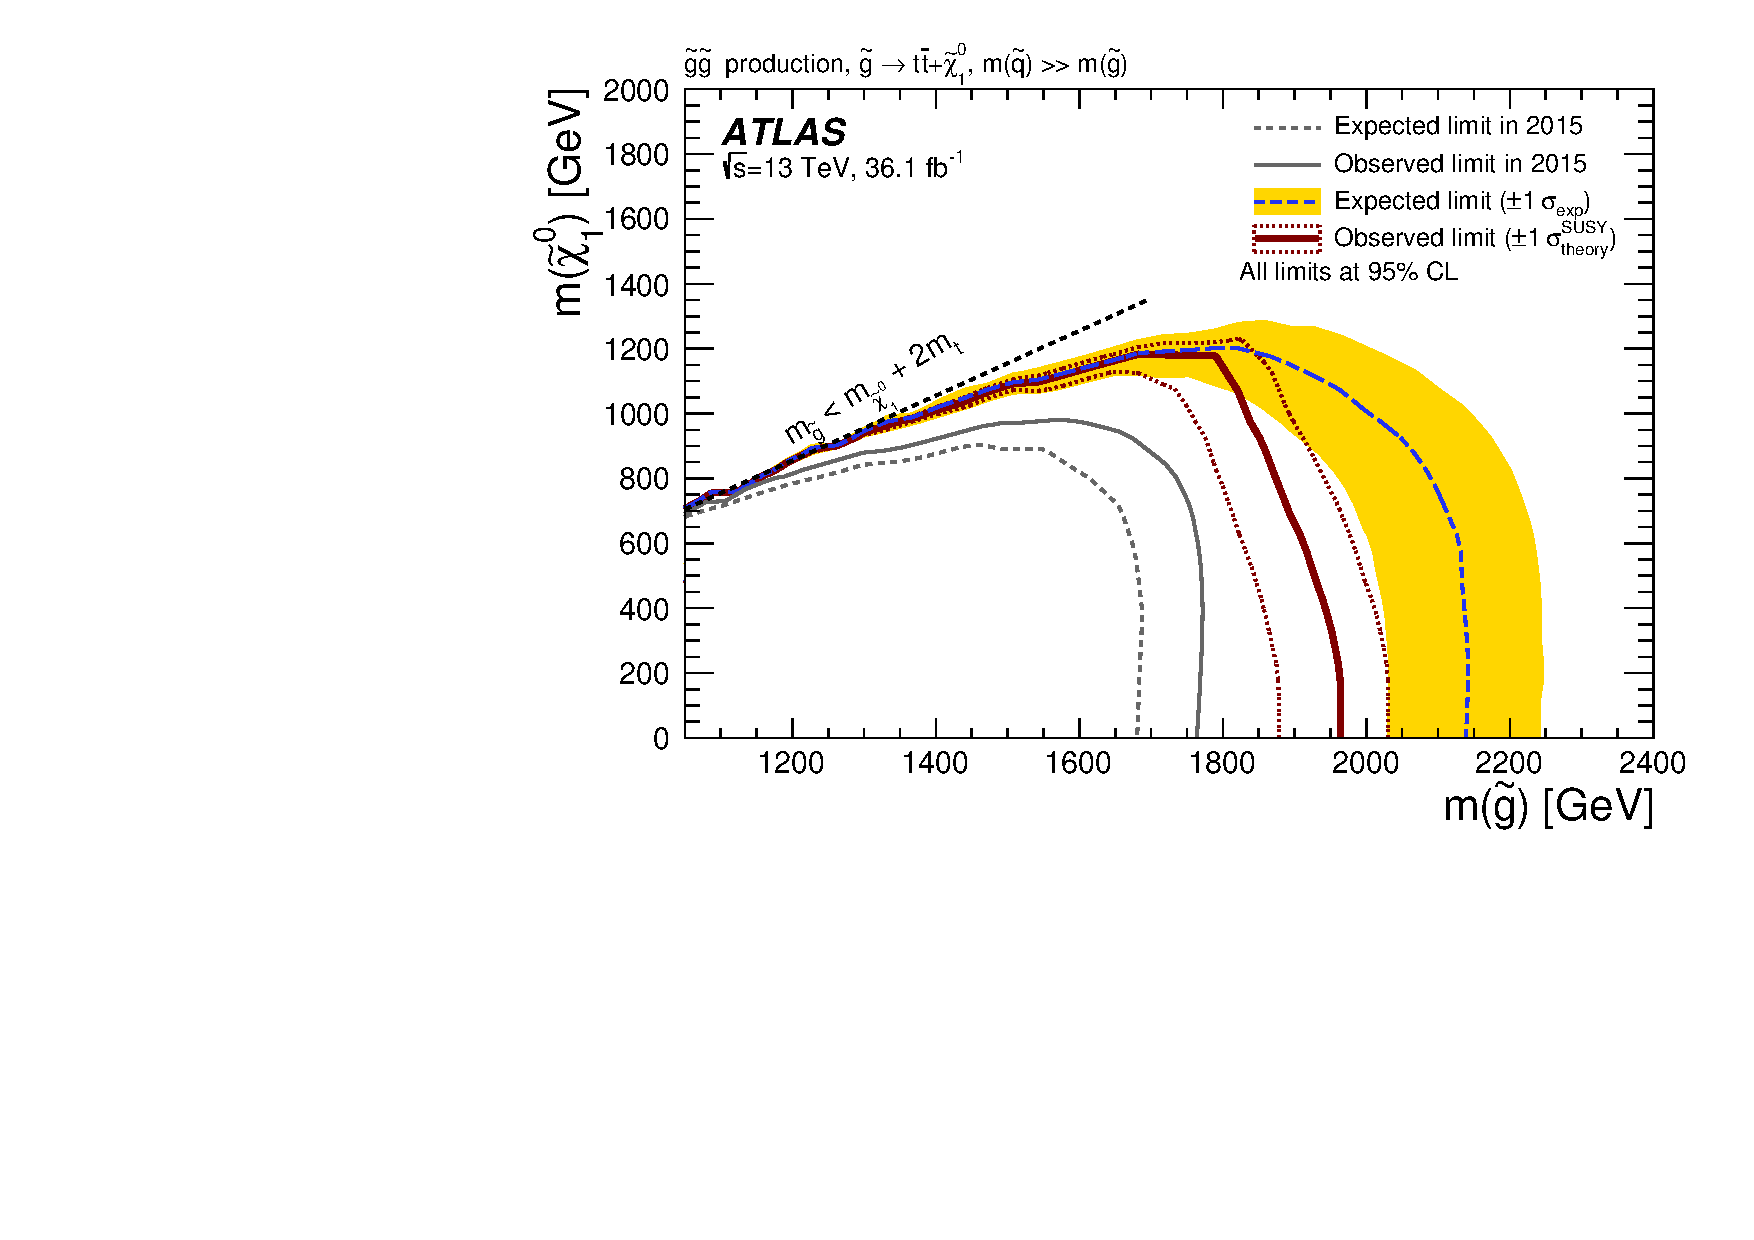
\includegraphics[width=0.65\textwidth]{figures/strong_prod/paper/limits/Limits_Gtt.pdf}\label{fig:limits_Gtt}}
	\subfigure[]{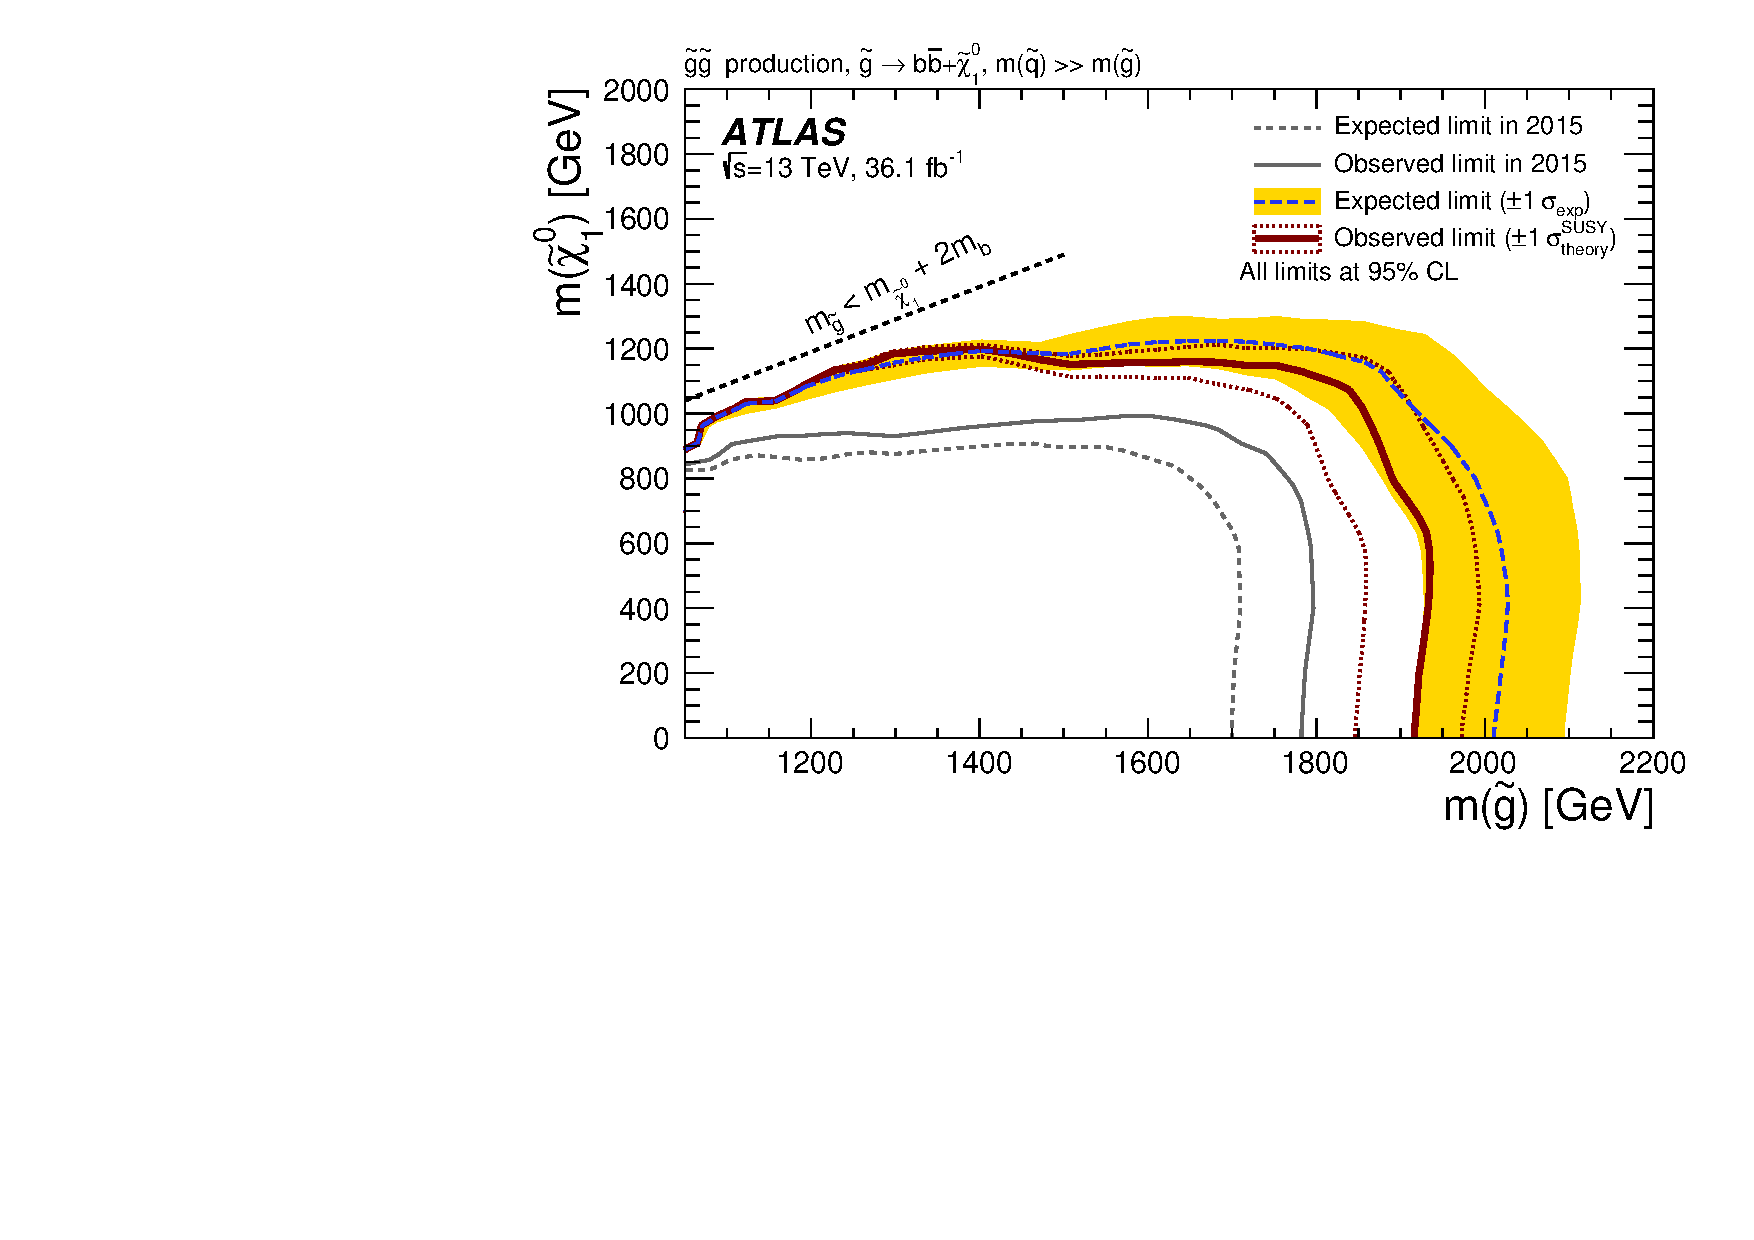
\includegraphics[width=0.65\textwidth]{figures/strong_prod/paper/limits/Limits_Gbb.pdf}\label{fig:limits_Gbb}}
	\caption{Exclusion limits in the $\ninoone$ and $\gluino$ mass plane
  		for the \subref{fig:limits_Gtt} Gtt and  \subref{fig:limits_Gbb} Gbb models obtained
		in the context of the multi-bin analysis. The dashed and solid bold lines
		show the 95\% CL expected and observed limits, respectively. The
  		shaded bands around the expected limits show the
                impact of the
  		experimental and background uncertainties. The dotted
  		lines show the impact on the observed limit of the variation of the
  		nominal signal cross-section by $\pm 1 \sigma$ of its theoretical
  		uncertainty. 
		The 95\%~CL expected and observed limits from the ATLAS search based on 2015 data 
  		\cite{Aad:2016eki} are also shown.}
	\label{fig:limits_GbbGtt}
\end{figure}


\begin{figure}[htbp]
	\centering
	\subfigure[]{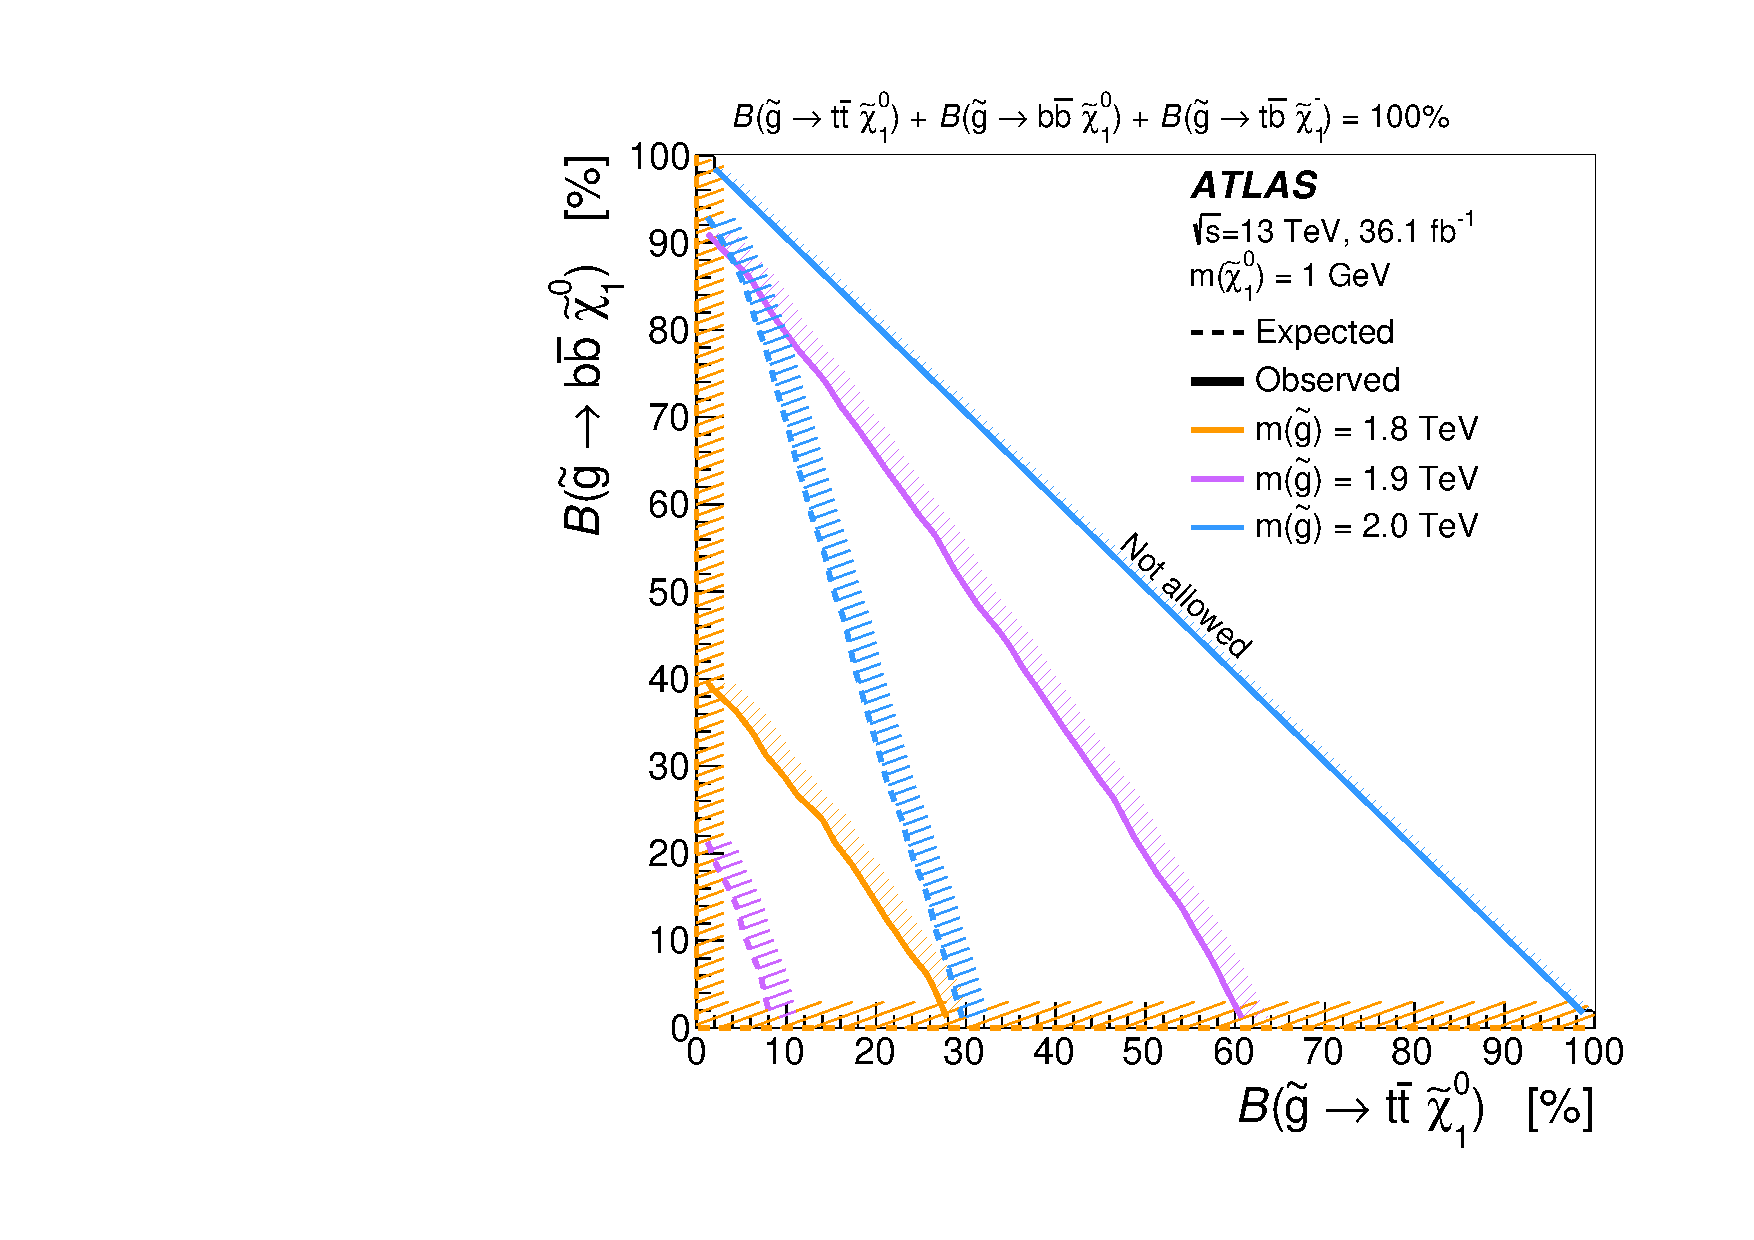
\includegraphics[width=0.65\textwidth]{figures/strong_prod/paper/limits/triangle_UL_massless_neutralino.pdf}\label{fig:limit_br_fixed_neu}}
	\subfigure[]{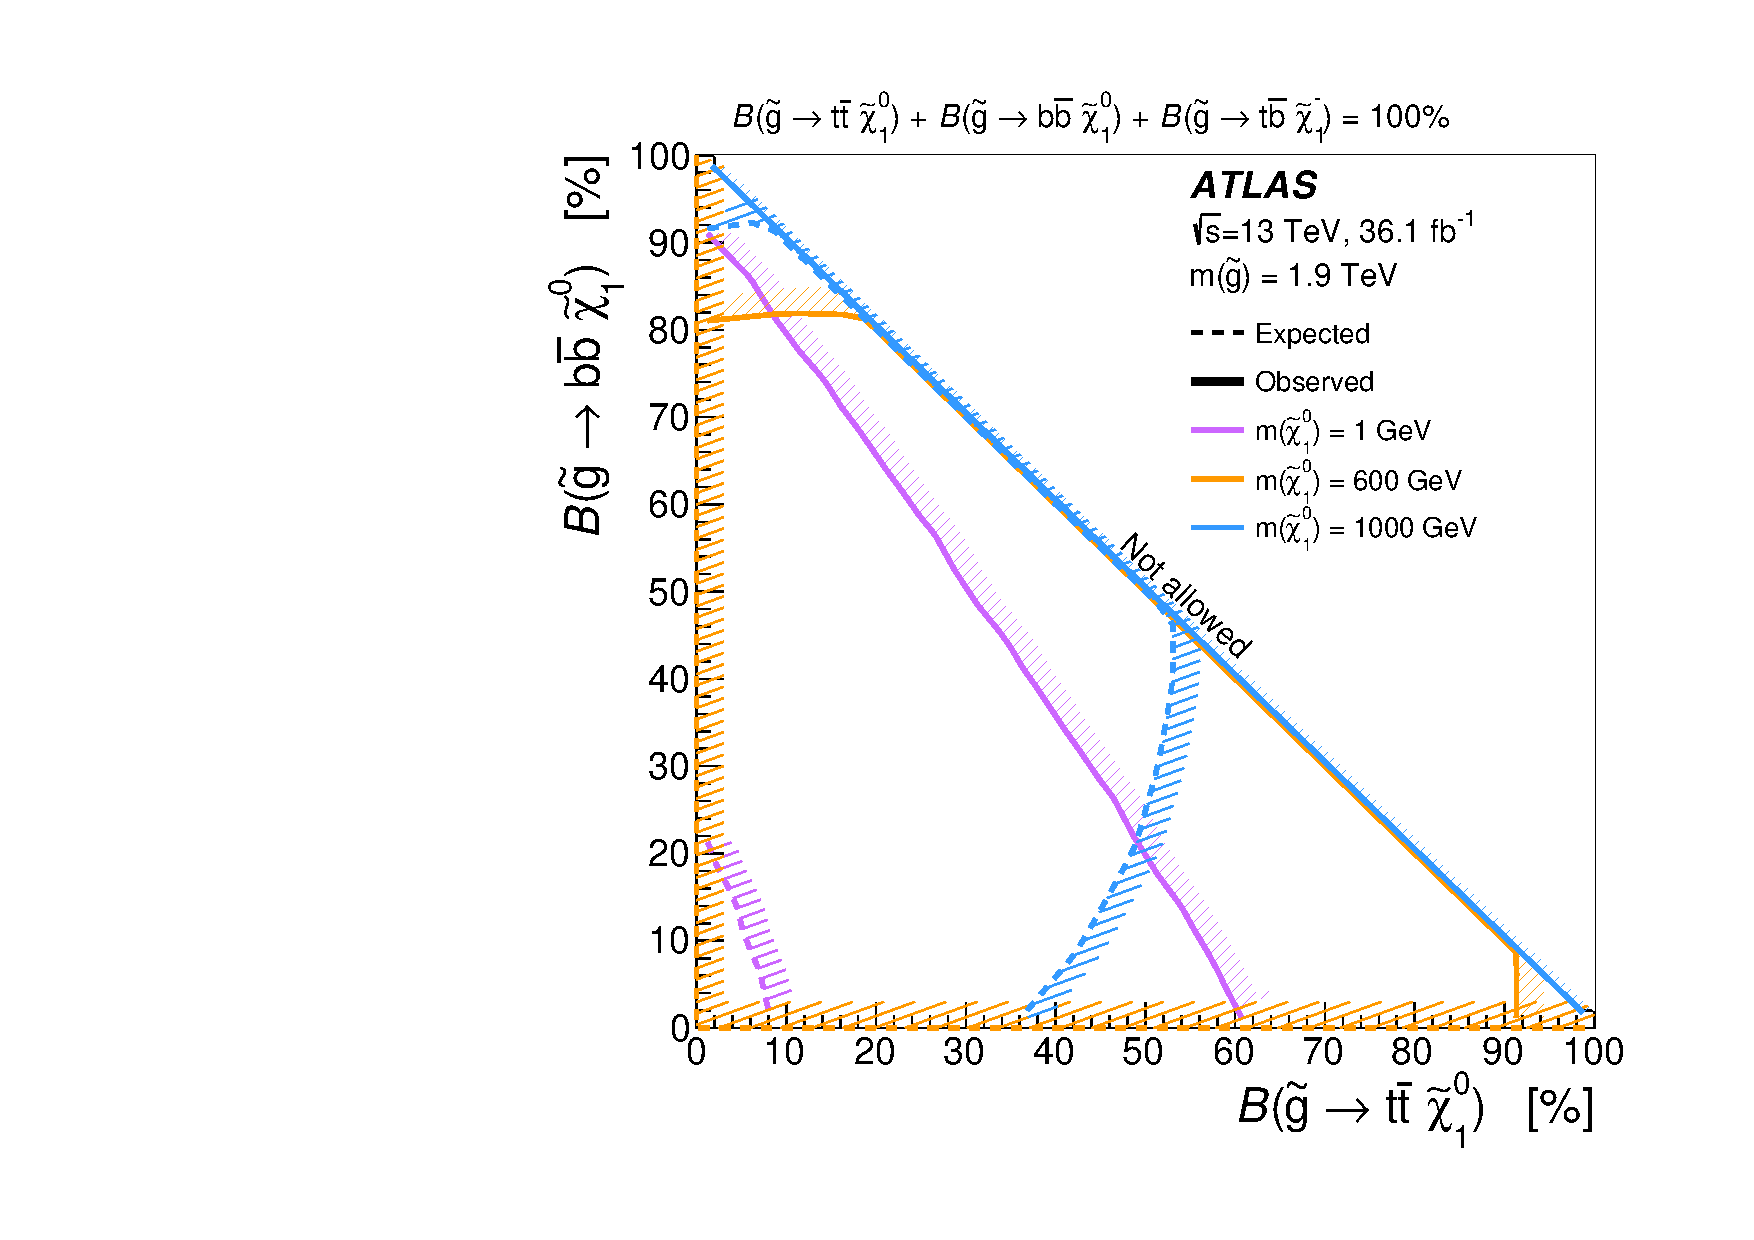
\includegraphics[width=0.65\textwidth]{figures/strong_prod/paper/limits/triangle_UL_1900_gluino.pdf}\label{fig:limit_br_fixed_glu}}
	\caption{Exclusion limits in the $\gluino \to t \bar{t} \ninoone$ and $\gluino \to b \bar{b} \ninoone$
		branching ratio plane assuming \subref{fig:limit_br_fixed_neu} a neutralino mass of 1 GeV and various gluino masses 
		(1.8, 1.9 and 2.0 TeV) and \subref{fig:limit_br_fixed_glu} a gluino mass of 1.9 TeV and three neutralino masses (1, 600 and 1000 GeV). 
		In \subref{fig:limit_br_fixed_neu}, the expected limit for a gluino mass of 1.8 TeV follows the plot axes, meaning that the whole plane is 
		expected to be excluded at 95\% CL.
		The dashed and solid bold lines show the 95\% CL expected and observed limits, respectively. The hashing indicates which side of the line 
		is excluded. The upper right half of the plane is forbidden by the requirement that the sum of branching ratios does not exceed 100\%.}
\end{figure}

\section{Results in the context of the ATLAS SUSY group}
